\documentclass[times, utf8, diplomski, numeric]{fer}
\usepackage{booktabs}
\usepackage{tikz}
\usepackage{graphicx}
\usepackage{amsmath}
\usepackage{bm}
\usepackage[]{mcode}
\usepackage{subcaption}
\usepackage{caption}
\usepackage{fancyhdr}
\usetikzlibrary{shapes,arrows}
\graphicspath{ {images/} }

\begin{document}
\tikzstyle{block} = [draw, fill=white!20, rectangle, 
    minimum height=2em, minimum width=4em]
\tikzstyle{block2} = [draw, fill=white!20, rectangle, 
    minimum height=0.1em, minimum width=0.1em]    
\tikzstyle{block_small} = [draw, fill=white!20, rectangle, 
    minimum height=2em, minimum width=2em]
\tikzstyle{sum} = [draw, fill=white!20, circle, node distance=2cm]
\tikzstyle{input} = [coordinate]
\tikzstyle{output} = [coordinate]
\tikzstyle{pinstyle} = [pin edge={to-,thin,black}]

% TODO: Navedite broj rada.
\thesisnumber{3962}

% TODO: Navedite naslov rada.
\title{Teleoperacija robotske ruke Kinova Jaco 3D kamerom}

% TODO: Navedite vaše ime i prezime.
\author{Filip Marić}

\maketitle

% Dodavanje zahvale ili prazne stranice. Ako ne želite dodati zahvalu, naredbu ostavite radi prazne stranice.
\zahvala{}

\tableofcontents

\chapter{Uvod}
Klasična upravljačka sučelja za robotske manipulatore kao što su tipkovnice ili daljinski upravljači u uporabi su od samih početaka razvoja robotike.
Kao pozitivna zajednička karakteristika ovih sučelja mogla bi se navesti njihova jednostavnost izvedbe: stisak odgovarajuće kombinacije tipki ili guranje kontrolne palice uzrokuje neku radnju manipulatora.
Dok su se ovakva sučelja pokazala efektivnim i cijenovno povoljnim rješenjem za ustaljene uloge robotskih manipulatora u industriji, njihov učinak u novijim primjenama ostavlja prostora za drugačije pristupe.

Zahvaljujući masovnoj proizvodnji tehnologija koje su za početka razvoja robotike bile u povojima, danas je prostor za razvoj inovativnih pristupa upravljačkim sučeljima veći nego ikad.
Robotski manipulatori vrlo su često anatomski slični ljudskoj ruci, što nas je dovelo do zaključka kako bi upravljanje ljudskom rukom rezultiralo visokom razinom intuitivnosti, čiji manjak smatramo glavnim nedostatkom klasičnih sučelja.

Zamišljeno upravljačko sučelje razlikuje se od klasičnih po još jednoj osnovnoj karakteristici: ne zahtjeva kontakt između opreme i korisnika.
Ovakav sustav ostvarujemo snimanjem pokreta ruke korisnika pomoću 3d kamere, koja uz sve funkcije standardne kamere vraća informaciju o udaljenosti objekata u kadru.
Dobivene informacije obrađuju se razvijenim algoritmom detekcije dlana ruke te se šalju preko mreže na upravljačko računalo robotskog manipulatora, koje ih pretvara u naredbe.


%doradi zadnji paragraf, bolje primjene, fokusirati se više na potrebu za ljudskim aspektom i postupnim ulaskom robota u svakodnevni život
Korisnost ovakvog sustava pronalazimo u širokom spektru područja, od vojne do zabavne industrije. 
U industriji zabave jedna moguća primjena je pomicanje kamere na kraju više-osnog manipulatora, gdje ovakvo upravljanje omogućuje intuitivniju kontrolu kadra od strane snimatelja.
Ljudima s poteškoćama u kretanju robotska ruka upravljana ovakvom metodom može olakšati dohvaćanje objekata u okolini. 
Ovakvim upravljanjem dobivamo prirodnije kretanje robotskih manipulatora, što će postupnim ulaskom robota u svakodnevni život postati tražena karakteristika.


\section{Opći i specifični ciljevi rada}
Opći cilj našeg rada bio je razvoj upravljačkog sučelja koje kao ulaznu informaciju koristi isključivo gestikulacije i pomake ruke korisnika.
Zamišljeno sučelje mora biti jednostavno za savladati novom korisniku, intuitivno , pružiti odgovarajuću razinu preciznosti i pri tome zadržati relativno nisku cijenu.
Iz ovih smjernica proizlaze specifični ciljevi rada:
\begin{itemize}
\item Cijeli sustav mora biti izveden koristeći besplatne, open-source\footnote{\textbf{open-source} - čiji je izvorni kod i/ili nacrti (dizajn) dostupan javnosti na uvid, korištenje, izmjene i daljnje raspačavanje} tehnologije. 
Ovime osiguravamo ažurnost sustava kroz vrijeme te jednostavnije popravke i modifikacije.
\item Radi nedostatka open-source rješenja za detekciju ruke korištenom 3d kamerom, potrebno je razviti detekcijski algoritam koji uzima u obzir ograničenja korištene sklopovske podrške i potrebe sustava.
\item Open source izvedba zahtjeva korištenje robotskog operacijskog sustava ROS, u kojem izvodimo cijelokupni upravljački algoritam.
\item Sustav mora biti primjenjiv na bilo kojem manipulatoru sa 3 ili više osi. Ovo ukazuje na potrebu za programskim rješavanjem problema kinematike robota uz dostupnu opisnu datoteku i kompatibilnost sa najčešćim izvedbama ROS-API\footnote{\textbf{API} (\textit{engl. application programming interface}) - set programskih "blokova" razvijen sa svrhom olakšavanja komunikacije i upravljanja programskim ili sklopovskim sustavom} sučelja.
\item Sustav mora imati zadovoljavajuće dinamičko ponašanje, što zahtjeva testiranje kinematike i upravljačke petlje na simulaciji razvijenoj za potrebe rada.
\end{itemize}

Kako bi ostvarili ove ciljeve bilo je potrebno savladati metodologiju korištenja nekolicine programskih paketa i biblioteka, kao i riješiti problem međusobne kompatibilnosti brojnih komponenti sustava.
Komponente je potom trebalo uklopiti u strukturu upravljačke petlje visoke razine, pri tome vodeći računa o radnim frekvencijama korištenih sklopova.

\chapter{Izvedba}
%detaljan opis kako funkcioniraju "oba" načina upravljanja, eventualno ubaciti cardboard slike, slike upravljanja, slike detekcija gui, slike cijelokupnog sustava
U ovom poglavlju opisujemo zamišljeno upravljačko sučelje. 
Prvo potpoglavlje opisuje dva načina na koje upravljački algoritam bilježi kretnje ruke korisnika.
Drugo potpoglavlje sadrži pregled arhitekture cjelokupnog sustava i svrhe pojedinih komponenata. 

\section{Interpretacija pokreta}\label{2_1}
Samom prenošenju kretnji ljudske ruke na robota pristupili smo na dva načina: prvi ostvaruje praćenje ljudske ruke u stvarnom vremenu, dok se drugi bazira na načelu sličnom upravljanju kontrolnom palicom (\textit{engl. joystick}).

Praćenje ljudske ruke ostvarujemo "poistovjećivanjem" dlana korisnika s alatom na vrhu manipulatora. 
Pri početku upravljanja ljudska se ruka nalazi na sredini kadra i odgovarajućoj udaljenosti, ova početna pozicija poistovjećuje se sa trenutnom pozicijom alata manipulatora.
Pomicanjem dlana korisnik pomiče željenu poziciju alata manipulatora.
Upravljačka petlja "primjećuje" ovu razliku te svara upravljački signal kojim nastoji izjednačiti stvarnu i željenu poziciju manipulatora.

Druga izvedba oko početne pozicije korisnikove ruke formira kuglu.
Zadržavanjem dlana korisnika unutar kugle, upravljački algoritam zadržava vrh manipulatora u trenutnoj poziciji.
Pomicanjem dlana korisnika izvan kugle, upravljački algoritam pomiče vrh manipulatora u smjeru vektora udaljenosti dlana od središta kugle.
\begin{figure}
\centering
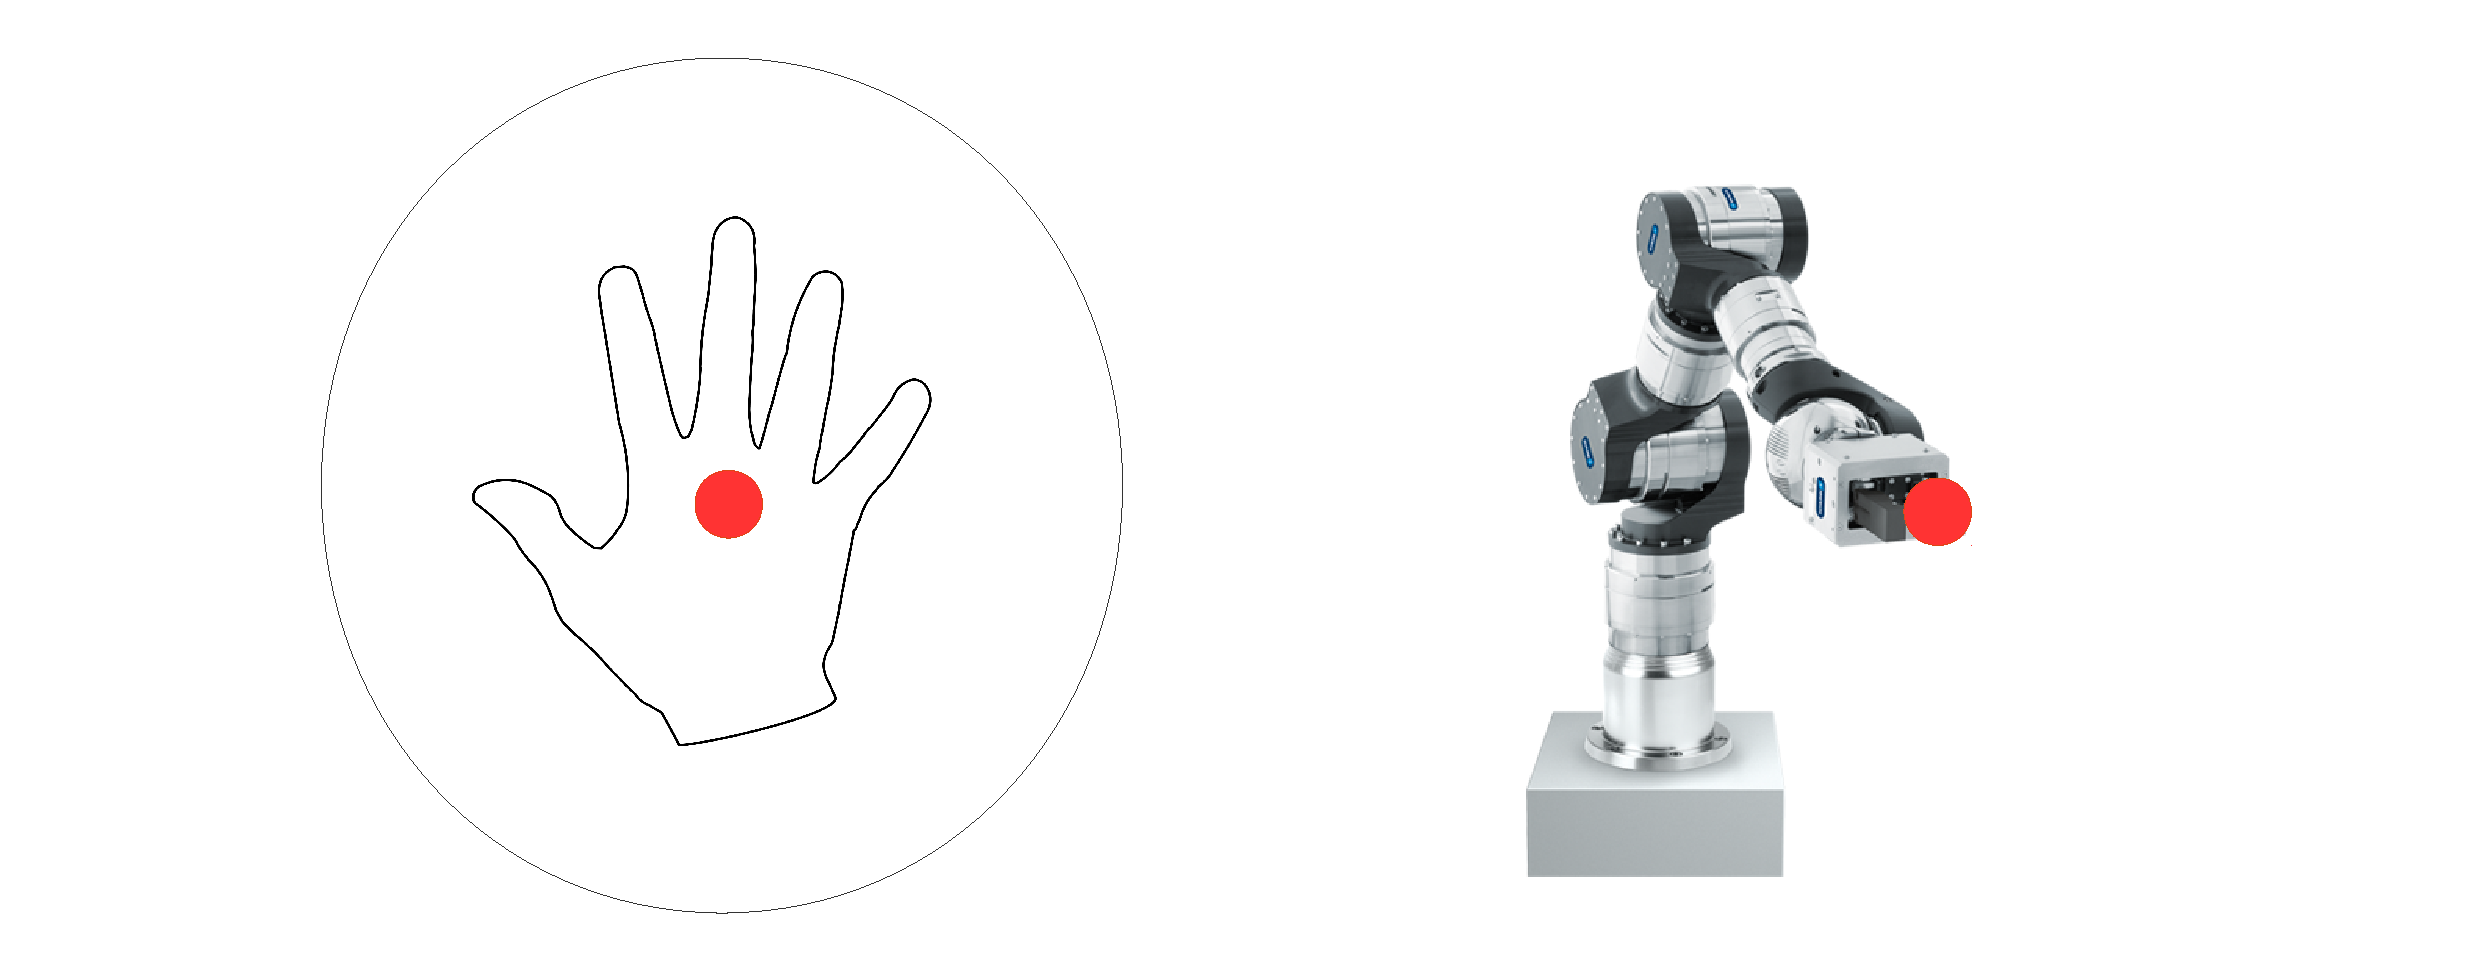
\includegraphics[scale=0.3]{koncept21}
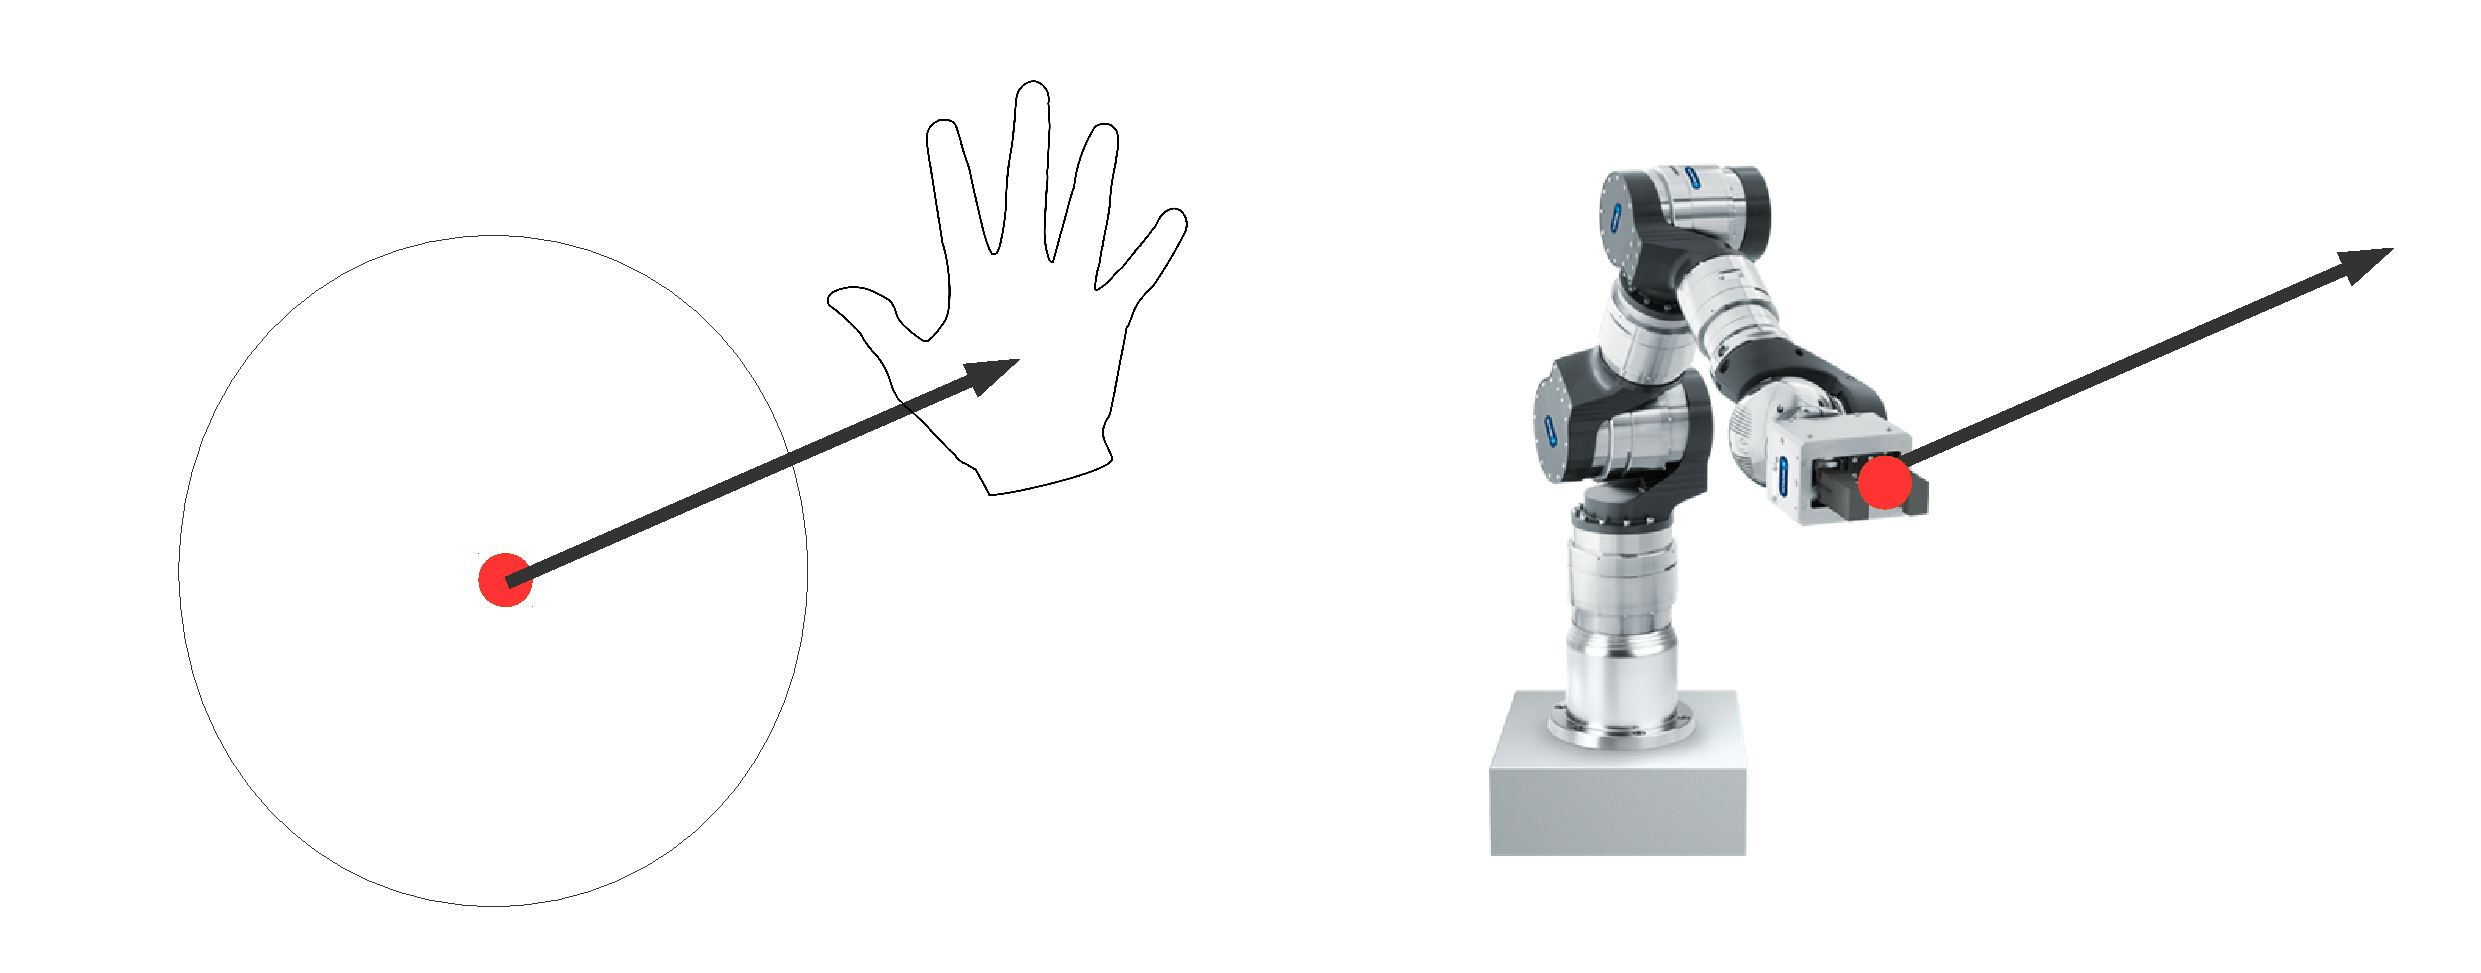
\includegraphics[scale=0.3]{koncept22}
\caption{Prikaz \textit{joystick} načina upravljanja.}
\end{figure}
Zajednička funkcija kod oba pristupa vezana je uz otvaranje i zatvaranje alata. 
Otvaranje šake korisnika upravljački algoritam interpretira kao naredbu otvaranja alata manipulaotra, dok se zatvorena šaka interpretira kao naredba zatvaranja.
Ova funkcija naravno ovisi o tipu alata na kraju manipulatora, no mapiranje otvaranja i zatvaranja šake na neku drugu funkciju nije komplicirano radi strukture podataka koji ulaze u upravljački algoritam.

\section{Struktura sustava upravljanja}
Sustav upravljanja na najvišoj se razini sastoji od 4 komponente:
\begin{itemize}
  \item \textbf{Detektor} Na dubinskoj RGBD slici pronalazi dlan korisnika i prostorne koordinate (i orijentaciju) njegove sredine. 
  \item \textbf{Regulator} Interpretira razliku trenutne pozicije (i orijentacije) dlana i izvršnog člana manipulatora. 
  Rezultat se pretvara u potrban zakret (ili brzinu zakreta) zglobova manipulatora, nakon čega se šalje u API sučelje.
  \item  \textbf{API sučelje} Prima upravljačku naredbu i nakon obrade je prosljeđuje na nižu razinu gdje se pretvara u API naredbu.
  U istom ciklusu API sučelje čita trenutna stanja zglobova manipulatora i šalje ih natrag prema regulatoru.
  \item  \textbf{Manipulator} Prima API naredbu te je pretvara u konkretna kretanja zglobova. 
  Ugrađeno sklopovlje bilježi senzorska očitanja sa zglobova te ih priprema za čitanje od strane API sučelja.
\end{itemize}

Kako bi kvalitetno ostvarili koncepte upravljanja navedene u potpoglavlju \ref{2_1}, vrlo nam je bitna povratna veza prikazana na slici \ref{izvedba}.
Povratna veza omogućuje nam uvid u trenutno stanje sustava čime se omogućuje ispravljanje pogrešaka, praćenje referentne veličine i otpornost na smetnje.
Pomoću informacija o poziciji pojedinačnih zglobova također osvježavamo matricu Jakobijana manipulatora, koja je ključni element općeg kinematičkog rješenja praćenja.

\begin{figure}[!h]
\centering
\begin{tikzpicture}[auto, node distance=3cm,>=latex']
    % We start by placing the blocks
    \node [block] (detekcija) {{\small Detektor}};
    \node [block, right of=detekcija] (Regulator) {{\small Regulator}};
    \node [block, right of=Regulator, node distance=3cm] (system) {{\small API sučelje}};
    % We draw an edge between the controller and system block to 
    % calculate the coordinate u. We need it to place the measurement block. 
    \draw [->] (Regulator) -- node[name=u] {} (system);
    \node [output, right of=system, node distance=3cm] (output) {};
    \node [block, below of=system, node distance=2cm] (measurements) {{\small Manipulator}};

    % Once the nodes are placed, connecting them is easy. 
    \draw [->] (detekcija) -- node {} (Regulator);
    \draw [->] (system) -- node [name=y] {}(output);
    \draw [->] (y) |- (measurements);
    \draw [->] (measurements) -| node[pos=0.99] {} 
        node [near end] {} (Regulator);
\end{tikzpicture}
\caption{Blok dijagram izvedbe sustava}\label{izvedba}
\end{figure}

\subsection{Detektor}
Zahtjevi postavljeni na detektor relativno su niski. 
Radna frekvencija trebala bi biti dovoljno visoka da pri prosječnom gibanju referentne veličine bivaju zadane prije no što ih manipulator može sustići.
Minimalni zahtjev na sam detekcijski algoritam jest mogućnost pronalaženja koordinata ljudskog dlana u barem dvije dimenzije, ovime se omogućava kretanje manipulatora po ravnini.
U našem radu izvedeno je trodimenzionalno translacijsko kretanje, dok je sustav potpuno osposobljen za detekciju punih 6 stupnjeva slobode gibanja.

\subsection{Regulator}
Pod pojmom regulator ovdje se podrazumjeva cijela programska struktura koja prima, obrađuje i šalje podatke između više objekata u stvarnom vremenu.
Stvarnu strukturu regulatora detaljnije ćemo razmotriti u poglavlju \ref{Upravljački algoritam}, kada se detaljnije upoznamo sa korištenom programskom podrškom i kinematičkim rješenjem.

Ovdje ćemo samo napomenuti da je za kvalitetan rad regulatora bitna sinkronizacija rada svih njegovih komponenti kako bi se ostvario stabilan protok podataka i stalna radna frekvencija sustava.
Ovo je ostvarujemo koristeći mrežnu arhitekturu operacijskog sustava ROS, koji omogućuje određivanje radne frekvencije komponenti i daje detaljan uvid u protok podataka.
Također, mrežna arhitektura ROS-a omogućuje pokretanje komponenti pojedinačno na različitim fizičkim računalima, što ide u prilog modularnosti sustava.

\subsection{API sučelje}
Općenitost sustava zahtjeva razdvajanje općih funkcija za regulaciju i obradu podataka od funkcija povezanih uz specifični korišteni manipulator.
Konkretnije, ovu komponentu moramo ostvariti tako da se na nju može spojiti API bilo kojeg manipulatora koji zadovoljava fizičke zahtjeve.

Paket \verb|ros_control| ostvaruje zadano sučelje koristeći apstraktne klase na koje "spajamo" API manipulatora.
Dovoljno je funkcije čitanja stanja zglobova i zadavanja brzine/pozicije "zamotati" u ponuđene klase, te ostatak sustava izvesti koristeći njih.

\subsection{Manipulator}
Manipulator je robotski uređaj koji izvršava željenu radnju te je na njega postavljeno nekoliko osnovnih zahtjeva kako bi bio kompatibilan sa sustavom.
Kao što je ranije spomenuto, sam manipulator mora imati minimalno dva računalom upravljiva stupnja slobode (time ostvarujemo planarno kretanje).
Također, manipulator mora biti opermljen senzorima pozicije i/ili brzine koje je moguće čitati na računalu koristeći API.

\chapter{Sklopovska podrška}

\section{Microsoft Kinect 3d kamera}

\section{Kinova Jaco robotska ruka}
Kinova Jaco (\ref{JACO2}) robotska je ruka namijenjena osobama s poteškoćama u kretanju.
Jaco 2010. godine na tržište je stavlja kanadska tvrka Kinova robotics s ciljem olakšavanja svakodnevnog života korisnika.
Manipulator ima 6 stupnjeva slobode, čime se ostvaruje puna sloboda pozicioniranja alata u prostoru.
Alat se sastoji od grabilice sa 3 prsta, što omgućuje stabilne hvatove velike količine svakodnevnih objekata.
Ruka je dizajnirana kako bi bila kompatibilna sa raznim dostupnim električnim invalidskim kolicima, ali je zbog svoje kvalitetne izrade i specifikacija našla široku primjenu u znanosti.

\begin{figure}[h!]
\centering
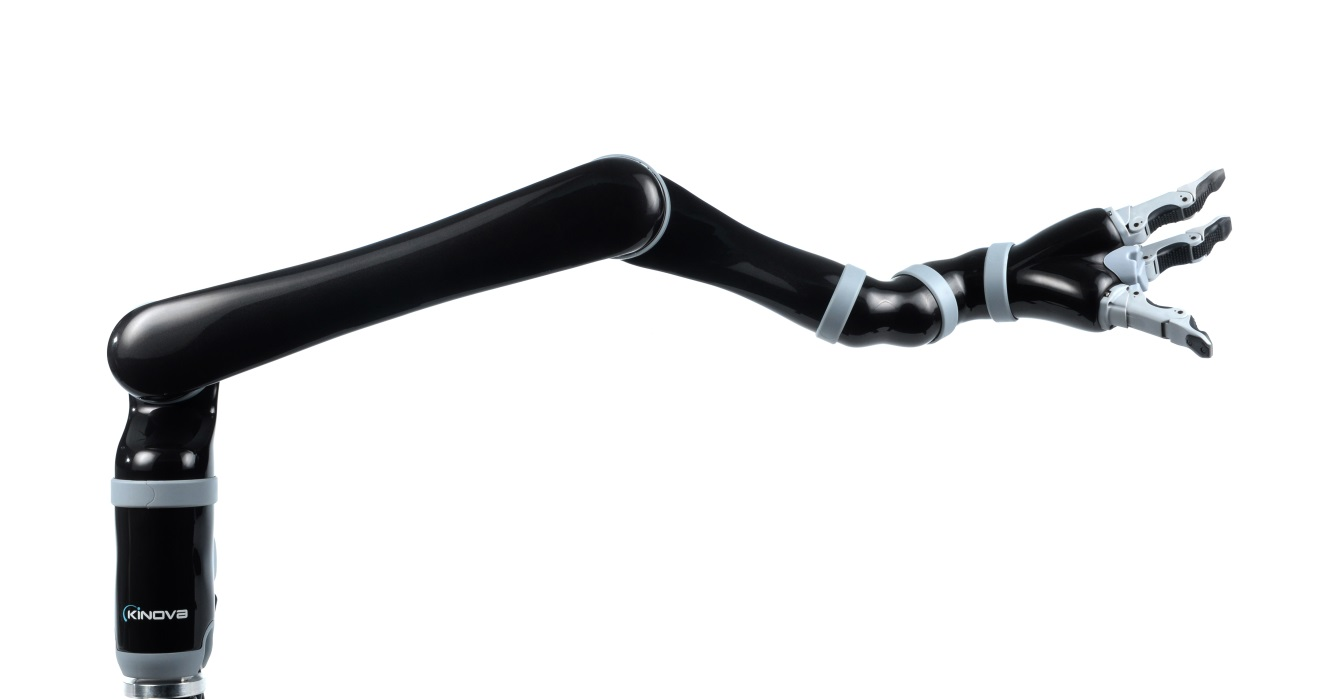
\includegraphics[width = 0.7\textwidth]{JACO2}
\caption{Kinova Jaco robotska ruka} \label{JACO2}
\end{figure}

\subsection{Tehničke specifikacije}
Glavne prednosti Jaco robotske ruke su relativno niska potrošnja električne energije i malena masa komponenata.
Aktuatori na zglobovima opremljeni su raznim senzorima kroz koje korisnik može dobiti veliku količinu povratnih informacija o stanju manipulatora.


\subsubsection{Opće specifikacije}
Potrebni ulazni napon kreće se od 18V do 29V,  a to su vrijednosti lako ostvarive baterijom ugradivom u električna invalidska kolica.
Masa od 5.6 kg osigurava jednostavnu montažu i sigurnost pri upravljanju, što je također vrlo bitno za primarnu svrhu ove robotske ruke.
Detaljan prikaz općih specifikacija manipulaotra nalazi se u tablici \ref{jaco_spec}.

\begin{table}[h!]
    \centering
    \begin{tabular}{ | l | l | l |}
    \hline
    Masa & $5.6 \pm 5\%$ [kg] \\ \hline
    Ulazni napon  & $18 - 29$ [VDC] \\ \hline
    Ulazna struja & $2 - 10$ [A] \\ \hline
    Srednja snaga & $40$ [W] \\ \hline
    Frekvencija upravljanja & $100$ [Hz] \\ \hline
    Max. teret na alatu pri srednjoj ispruženosti & $1.5$  [kg]  \\ \hline
    Max. teret na alatu pri maksimalnoj ispruženosti  & $1$ [kg]\\ \hline
    Dohvat & $90$  [cm] \\ \hline
    Linearna brzina alata & $5 - 15$ [cm/s]\\ \hline
    Sila stiska prsta & $7$ [N] \\ \hline
    \end{tabular}
    \caption{Prikaz tehničkih specifikacija Jaco robotske ruke} \label{jaco_spec}
\end{table}

\subsubsection{Aktuatori}

Manipulator se sastoji od 2 grupe od 3 identična aktuatora, modela K-75+ i K-58.
Veći aktuatori (K-75+) čine 3 donja zgloba koji podnose najveće terete, dok manji aktuatori (K-58) zauzimaju mjesto zglobova čija je primarna funkcija postavljanje orijentacije alata u prostoru.
Postoje još 3 aktuatora koji preko mehanizma arhimedovog vijka pokreću prste. 
Detaljan pregled specifikacija aktuatora nalazi se u tablicama \ref{spec_act_big}, \ref{spec_act_small}, \ref{spec_act_finger}.

\begin{figure}[h!]
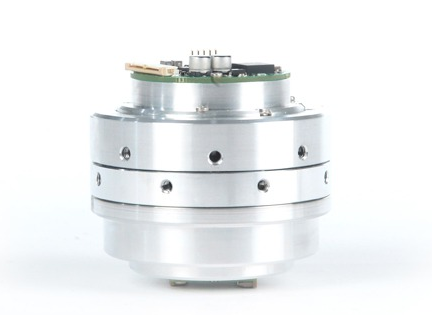
\includegraphics[scale=0.5]{k75plus}
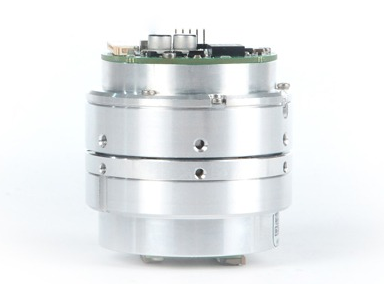
\includegraphics[scale=0.5]{k58}
\caption{a) aktuator K-75+ b) aktuator K-58}
\end{figure}

\begin{table}[h!]
    \centering
    \begin{tabular}{ | l | l | l |}
    \hline
    Masa & $0.64 \pm 2\%$ [kg] \\ \hline
    Promjer  & $74.5(+0.00/-0.03)$ [mm] \\ \hline
    Visina & $67$ [mm] \\ \hline
    Maksimalna brzina & $8$ [RPM] \\ \hline
    Apsolutna pogreška pozicije & $\pm0.5^{\circ}$ \\ \hline
    Ulazni napon  & $18 - 29$ [VDC] \\ \hline
    Nominalni moment & $15$ [Nm] \\ \hline
    Maksimalni moment & $26$  [Nm]  \\ \hline
    \end{tabular}
    \caption{Prikaz tehničkih specifikacija većih aktuatora.} \label{spec_act_big}
\end{table}

\begin{table}[h!]
    \centering
    \begin{tabular}{ | l | l | l |}
    \hline
    Masa & $0.39 \pm 2\%$ [kg] \\ \hline
    Promjer  & $58(+0.00/-0.03)$ [mm] \\ \hline
    Visina & $69$ [mm] \\ \hline
    Maksimalna brzina & $10$ [RPM] \\ \hline
    Apsolutna pogreška pozicije & $\pm0.5^{\circ}$ \\ \hline
    Ulazni napon  & $18 - 29$ [VDC] \\ \hline
    Nominalni moment & $4$ [Nm] \\ \hline
    Maksimalni moment & $7$  [Nm]  \\ \hline
    \end{tabular}
    \caption{Prikaz tehničkih specifikacija manjih aktuatora} \label{spec_act_small}
\end{table}

\begin{table}[h!]
    \centering
    \begin{tabular}{ | l | l | l |}
    \hline
    Maksimalna brzina & $600$ [RPM] \\ \hline
    Ulazni napon  & $18 - 29$ [VDC] \\ \hline
    Nominalni moment & $15$ [mNm] \\ \hline
    Maksimalni moment & $30$  [mNm]  \\ \hline
    \end{tabular}
    \caption{Prikaz tehničkih specifikacija aktuatora prstiju} \label{spec_act_finger}
\end{table}

\subsubsection{Senzori}
Jaco robotska ruka opremljena je velikom količinom senzora.
Svaki zglob posjeduje senzore pozicije, temperature, struje i napona.
                                                                                                                            
Senzori pozicije služe za bilježenje zakreta svakog pojedinačnog zgloba manipulatora, diferenciranjem zakreta dobivamo informaciju o brzini okretanja.
Informacijom o temperaturi aktuatora osiguravamo manipulator od moguće štete uzrokovane prekomjernim zagrijavanjem.
Pomoću senzora struje moguće je dobiti povratnu informaciju o momentu razvijenom na pojedinom aktuatoru, ovaj zaključak proizlazi iz dobro poznatog identiteta:
\begin{align}
m_m \approx k \ i_a;
\end{align}
Ovdje $i_a$ predstavlja trenutnu struju armature akturatora, dok je $k$ konstanta definirana specifikacijama motora.

\begin{figure}[h!]
\centering
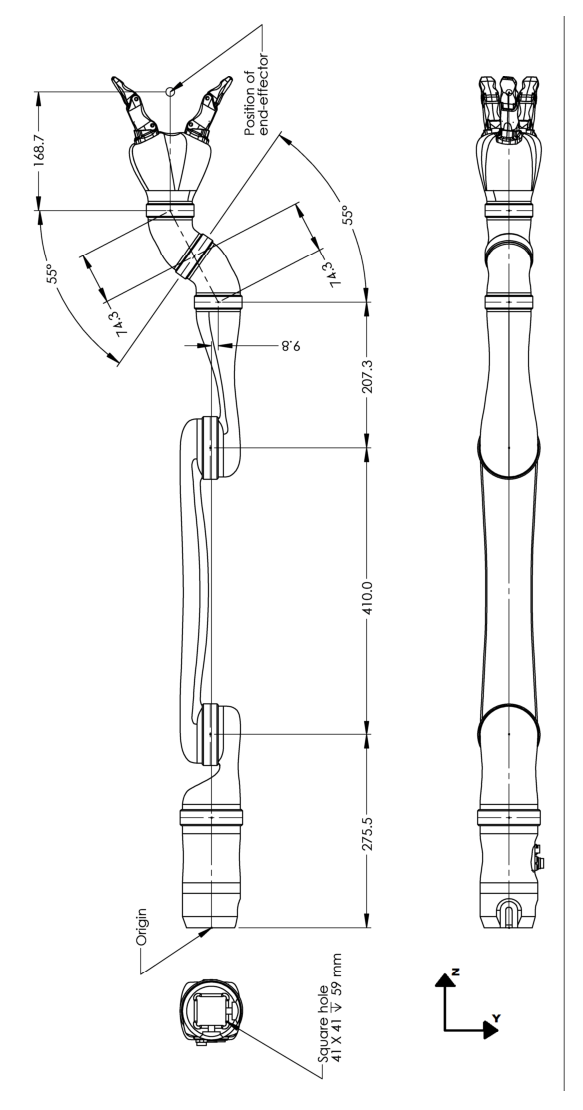
\includegraphics[width = 0.5\textwidth]{jaco_cad}
\caption{Shema Kinova Jaco robotske ruke sa označenim duljinama i zakretima elemenata}
\end{figure}

\subsection{Računalno sučelje}
Jaco robotska ruka s računalom se povezuje preko USB 2.0 (\textit{engl. Universal Serial Bus}) sučelja.
SDK\footnote{SDK (engl. Software Development Kit) - paket je programskih biblioteka, alata i uputa za razvoj vlastitih aplikacija za određeni programski ili sklopovski sustav.} Jaco robotske ruke kompatibilan je s novijim inačicama Linux Ubuntu i Windows operativnih sustava, a uz API sadrži grafičko upravljačko sučelje i bazu primjera korištenja API biblioteka.



\chapter{Programska podrška}
Ovo poglavlje sadrži opise svih programskih paketa, biblioteka i elemenata korištenih u ovom radu. 
Kratko opisujemo karakteristke i uloge svake pojedine stavke programskog dijela arhitekture sustava.
Potpoglavlja koja opisuju ROS i Gazebo sadrže nešto detaljnije opise, jer smatramo da je razumijevanje načela njihova rada ključno za razumijevanje načela rada sustava.

\section{ROS}
\begin{figure}[h!]
\centering

\includegraphics[width = 0.5\textwidth]{ros_enabled}
\caption{ROS logotip}
\end{figure}
ROS (engl. \textit{Robot Operating System}) je operacijski sustav koji omogućuje jednostavno povezivanja alata i biblioteka potrebnih za razne izvedbe u robotici. 
ROS je razvijen 2007. godine pod imenom \textit{switchyard} unutar laboratorija za umjetnu inteligenciju sveučilišta Stanford, kao razvojni alat za STAIR\footnote{\textbf{STAIR} - STanford Artificial Intelligence Robot} robota.
2008. godine razvoj ROS-a preuzima institut Willow Garage iz Kalifornije. 
Od 2013. na dalje ROS postaje potpuno open-source i razvoj preuzima Open Source Robotics Foundation.

Glavna gradivna jedinica svake izvedbe u ROS-u je paket.
Paketi u sebi sadrže C++/Python aplikacije koje nazivamo čvorovima (engl. \textit{nodes}).
Čvorove koristimo za komunikaciju s hardwareom (aktuatorima , senzorima ...), upravljanje simulacijama i prikazivanje podataka.
Izvedbe se u stvarnosti najčešće sastoje od više paketa, stoga se prava prednost ROS-a krije u ostvarivanju brze i učinkovite peer-to-peer komunikacije među čvorovima.
 
Komunikacija u ROS-u ostvaruje se mrežno (TCP/IP i UDP/IP protokolom) pomoću tema (engl. \textit{topics}) i poruka (engl. \textit{messages}).
Uz gore navedeno, ROS nudi razne naredbe unutar terminala koje olakšavaju prikaz podataka te dijagnostiku pri uklanjanju pogrešaka u kodu. Treba napomenuti da postoje i druge opcije za izvedbu aplikacija u robotici , kao što je OROCOS (engl. \textit{Open Robot Control Software} ). ROS je za ovaj projekt izabran zbog jednostavnosti izvedbe i postojećih paketa za JACO robotsku ruku.
\subsection{Osnovni koncepti}
Osnovna komunikacija u ROS-u može se vizualizirati u obliku grafa povezanih čvorova i tema. Ovakva struktura daje praktičan način prikazivanja sustava na najvišoj razini, čime se olakšava programska izvedba logike upravljanja. 

\begin{figure}[h!]
\begin{center}
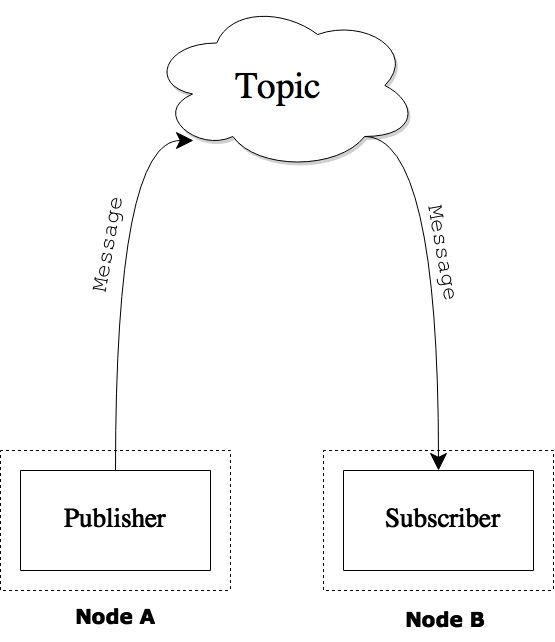
\includegraphics[scale=0.41]{Zavrsni_ROS}
\caption{Node A i Node B ostvaruju jednosmjernu komunikaciju koristeći topic}
\end{center}
\end{figure}

Čvorovi spremaju podatke u standardizirane strukture koje zovemo porukama te ih objavljuju na odgovarajuće mrežne lokacije koje nazivamo temama. 
Svaka tema prima samo jednu točno definiranu vrstu poruke. 
Objavljivač (en. \textit{publisher}) je objekt koji unutar čvora šalje poruku na temu, dok pretplatnik (en. \textit{subscriber}) čini njegov komplement i čita poruku s teme.

Ovaj način komunikacije omogućuje distribuciju raznih procesa na više računala što izvedbe čini manje ovisnima o sistemskim zahtjevima i izboru programskog jezika za pojedine čvorove. 
%slika streama jednog topica

\subsection{Ostale korištene funkcionalnosti}
Uz navedene osnovne funkcionalnosti , ROS sadrži neke složenije koncepte od kojih ćemo ovdje izdvojiti servise i parametarski server. 

\subsubsection{Servisi}
U ovom radu koriste se servisi (engl. \textit{services}). 
Pomoću servisa čvor A može direktno zahtijevati odgovor čvora B preko mreže. 
Čvor A objavljuje servis na mrežnu lokaciju sličnu temi, na tu lokaciju čvor B šalje zahtjev i adresu za spremanje odgovora. 
Čvor A učitava zahtjev s mrežne lokacije, obrađuje ga i odgovor sprema na adresu.

Zahtjev i odgovor najčešće su standardne ROS poruke, što znači da se pomoću servisa omogućuje korištenje funkcija čvora A u čvoru B. 
Ova funkcionalnost vrlo je korisna za distribuirane izvedbe procesno intenzivnih zadataka. 

\subsubsection{Parametarski server}
Parametrima (engl. \textit{parameters}) nazivamo karakteristične veličine unutar ROS čvorova koje se koriste pri izračunima varijabli. 
Glavna razlika između parametra i varijable nalazi se u frekvenciji promjene, koja je za parametre znatno niža. 

ROS nudi mogućnost učitavanja parametara s mrežnih lokacija čime se omogućuje jednostavno fino podešavanje ponašanja čvora pri testiranju.
Ovakvim pristupom se izbjegava potreba ponovnim kompiliranje koda pri svakoj promjeni parametara.

\subsection{ros control}
ROS paket \verb|ros_control| ostvaruje generičke PID regulatore unutar ROS arhitekture. 
Jednostavna i standardizirana integracija s ostatkom ROS ekosustava čini ovaj paket čestom komponentom sustava izvedenih u ROS-u.

Kako bi se postiglo poopćenje PID upravljanja neovisno o konkretnom robotu (tj. o API-ju), API funkcije robota "umataju" se unutar apstraktnih funkcija koje čine ROS-API sučelje.
Umjesto da regulatori šalju i čitaju podatke koristeći API funkcije direktno, ove operacije obavljaju se na generičkim funkcijama unutar kojih su "umotane" API funkcije .
Ovime korisnik kako bi primjenio postojeći sustav na drugog robota mora samo uklopiti odgovarajuće API funkcije unutar generičkih.
Za dobar dio robota ovo sučelje već postoji radi open-source karaktera ROS ekosustava.

\begin{figure}[h!]
\centering
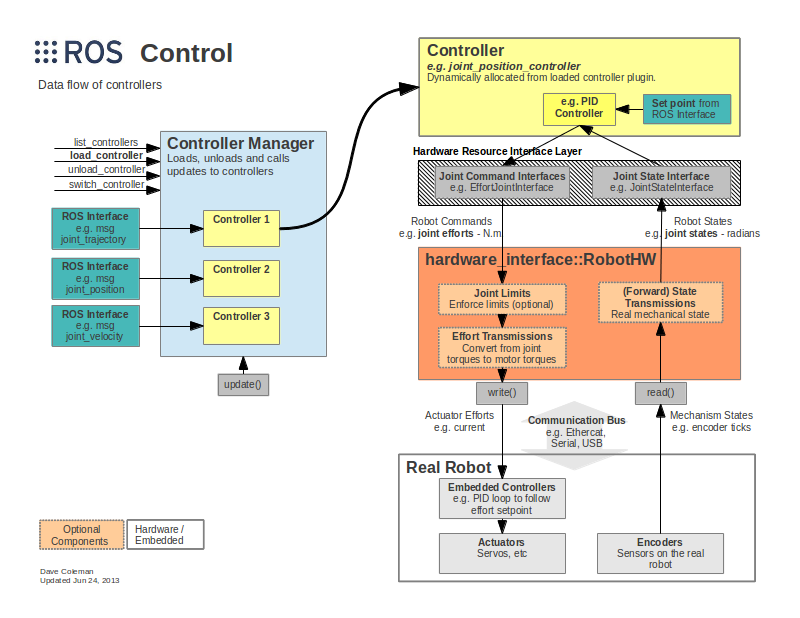
\includegraphics[scale=1]{gazebo_ros_control}
\caption{Mathworks Matlab logo}
\end{figure}

\section{Matlab}
\begin{figure}[h!]
\centering
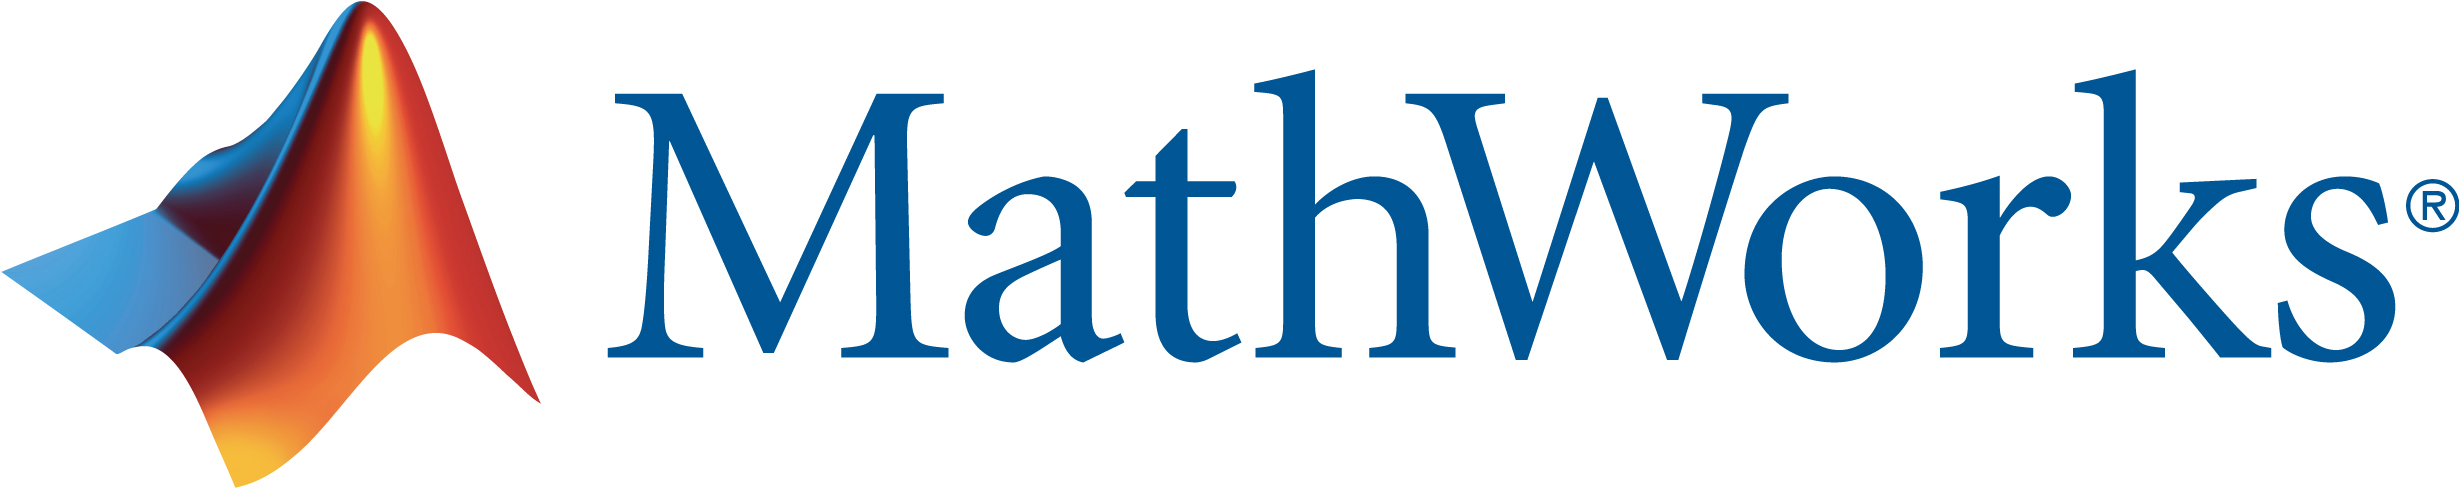
\includegraphics[scale=0.4]{logo_mathworks}
\caption{Mathworks Matlab logo}
\end{figure}
Matlab je računalno okruženje namjenjeno rješavanju širokog spektra tehničkih, računalnih i znanstvenih problema.
U užem smislu Matlab je viši programski jezik četvrte generacije koji omogućava manipulaciju matricama, numeričko računanje, iscrtavanje funkcija i još velik broj korisnih aplikacija.
Unutar Matlaba nalazi se veliki broj programskih paketa koji se koriste za specifične probleme, a nama je bitan paket za simbolički račun.
U ovom radu Matlab koristimo pri razvoju rješenja kinematike robotske ruke.

\section{OpenCV}

\section{KDL}
KDL (engl. \textit{Kinematics Dynamics Library}) je open-source C++ biblioteka razvijena za modeliranje i računanje kinematičkih lanaca.
Pomoću ove biblioteke moguće je jednostavno programski rješavati direktnu i inverznu kinematiku te dinamiku manipulatora sa manje od 7 stupnjeva slobode.
Nama je vrlo korisna mogućnost konstrukcije Jacobijeve matrice manipulatora (definirana kasnije), čiji se pseudoinverz pokazuje vrlo važnim rješenju problema praćenja putanje u općem slučaju.
KDL također vodi računa o izbjegavanju singulariteta u matricama, čime je osiguran kontinuiran rad upravljačkog algoritma.

\section{Gazebo}
\begin{figure}[h!]
\centering

\includegraphics[scale=0.5]{gazebo_1}
\caption{Gazebo logo}
\end{figure}
Gazebo je open-source programski paket za simulaciju robotskih sustava, njihovih senzora i okoline.
Kako bi se postiglo simuliranje dinamike robota , moguće je izabrati jedan od nekoliko modula koje Gazebo podržava.
Gazebo također omogućuje kvalitetno iscrtavanje 3d modela korištenog robota pomoću OGRE 3d modula.

Semantički opis robota, njegovih komponenti, prijenosa i zglobova Gazebo dobiva iz pripadajuće URDF datoteke.
URDF je vrlo često korišten format za opis kinematičkih lanaca koji nudi kvalitetnu integraciju u sa Gazebom i brojnim drugim robotičkim aplikacijama.
Gotovo svaki komercijalni robotski manipulator ima pripadajuću URDF datoteku i ta nam činjenica omogućuje izradu univerzalnog upravljačkog sučelja.


\subsection{ROS integracija Gazebo paketa}
Glavni razlog za korištenje ovog simulacijskog paketa uska je integracija sa ROS-om , čime postižemo jednostavan transfer sustava razvijenog na simulaciji na stvarni manipulator.
Gazebo simulaciju moguće je potpuno upravljati kroz ROS koristeći \verb|ros_control| sučelje, na isti način kao što upravljamo stvarnim sustavom.
Ova kompatibilnost ostvaruje se kroz \verb|gazebo_ros|, \verb|gazebo_msgs|, \verb|gazebo_plugins|  ROS pakete.
Ros control sučelje simulacije definiramo unutar URDF datoteke te se pri pokretanju Gazeba unutar ROS okruženja ono objavljuje kao stvarno.
Zahvaljujući ovoj činjenici, sustav možemo razvijati za simulaciju i stvarni sustav istovremeno, što se pokazalo vrlo korisnim.





\chapter{Kinematika manipulatora}
Modularna arhitektura našeg sustava dopušta integraciju manipulatora sa različitim razinama kompleksnosti API-ja.
Unatoč tome što većina komercijalnih manipulatora dolazi sa već izvedenim kinematičkim funkcijama, smatramo da je radi kompletnosti izvedbe bitno pripremiti sustav i za slučaj kada su dostupne samo naredbe pomicanja zglobova.
Ovo poglavlje prikazuje teoretsku pozadinu programskog rješenja kinematike manipulatora izvedenog unutar našeg sustava na relativno složenom primjeru Jaco robotske ruke.
Kinematičko rješenje nakon toga provjeravamo na dinamičkoj simulaciji ruke u programskom paketu Gazebo.

\begin{figure}[h!]
\centering
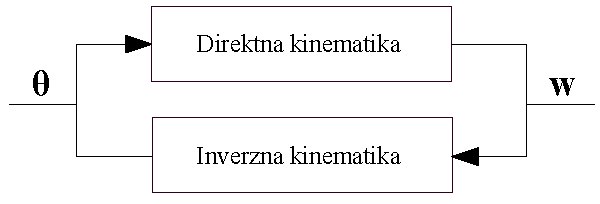
\includegraphics[scale=0.8]{kinematika}
\caption{Model Jaco robotske ruke sa označenim parametrima} \label{h}
\end{figure}

U idealnom slučaju, rješavanje problema kinematike manipulatora sa do 6 stupnjeva slobode zahtjeva sintezu matrica homogene transformacije između koordinatnih sustava baze i alata.
Iz članova dobivene matrice potom analitički dobivamo izraze za Kartezijsku poziciju i orijentaciju alata u ovisnosti o zakretima zglobova.
Sintezu direktne kinematike započinjemo D-H postupkom postavljanja koordinatnih sustava vezanih uz zglobove.
Određivanjem matrica homogenih transformacija između tih sustava dobivamo bijektivnu\footnote{Uz pretpostavku restrikcije zakreta zglobova na vrijednosti $[0,2\pi]$.} funkciju koja prostor zglobova preslikava u 6-dimenzionalni prostor pozicije.

Problem inverzne kinematike znatno je složeniji jer zahtjeva rješavanje sustava nelinearnih jednadžbi s više nepoznanica.
Za složenije manipulatore ovaj problem je netrivijalan te rješenje nije uvijek moguće pronaći koristeći osnovne matematičke metode.
Još jedna otežavajuća okolnost nalazi se u činjenici da će dobivena rješenja često biti višestruka, a pronalaženje odgovarajućeg ovisi o konstrukciji i poziciji manipulatora.

Pronalaženje analitičkih rješenja inverzne kinematike pomoću računalnog algoritma još je složeniji zadatak jer zahtjeva implementaciju univerzalnog pristupa rješavanju nelinearnih jednadžbi čija su rješenja višestruka.
Pronašli smo da je ovaj problem moguće zaobići koristeći iterativnu metodu baziranu na pronalaženju (pseudo)inverza matrice Jakobijana manipulatora, koja je puno prikladnija za programsku izvedbu.

U prvom potpoglavlju opisati ćemo osnovne postupke rješavanja kinematičkog problema na primjeru Jaco robotske ruke.
Pri tome ćemo radi sažetosti izlaganja preskočiti pojedinosti D-H postupka i izvod matrica homogene transformacije.
Drugo potpoglavlje sadrži opis ideje rješenja inverzne kinematike koje koristimo u računalnom algoritmu.
Rezultate zamišljenog postupka potom ispitujemo koristeći Matlab.
\newpage
\section{Direktna i inverzna kinematika Jaco robotske ruke}
\subsection{Direktna kinematika}
Problem direktne kinematike rješavamo tako da prvo postavimo koordinatne sustave koji odgovaraju svakom pojedinačnom zglobu prema pravilima D-H postupka.
Iz međusobnih udaljenosti i razlika u orijentaciji ovih zglobova porizlaze D-H parametri koje koristimo za sintezu matrica homogenih transformacija.
Množenjem dobivenih matrica dobivamo matricu koja izražava poziciju i orijentaciju alata izražene Kartezijevim koordinatama u ovisnosti o zakretu zglobova.
 
\subsubsection{DH Parametri}
Pri sintezi matrica transformacije ruke korišteni su D-H parametri iz službene dokumentacije za Jaco robotsku ruku prikazani u tablici \ref{JacoDH}. 
Za sintezu D-H parametara koristimo duljine članaka kao i parametre koji su iz njih izvedeni, prikazani su na slici \ref{jacoparam}.
Parametre $d_{4b}$, $d_{5b}$ i $d_{6b}$ određujemo iz izraza \ref{d4b}, \ref{d5b}, \ref{d6b}.
\begin{figure}[h!]
\centering
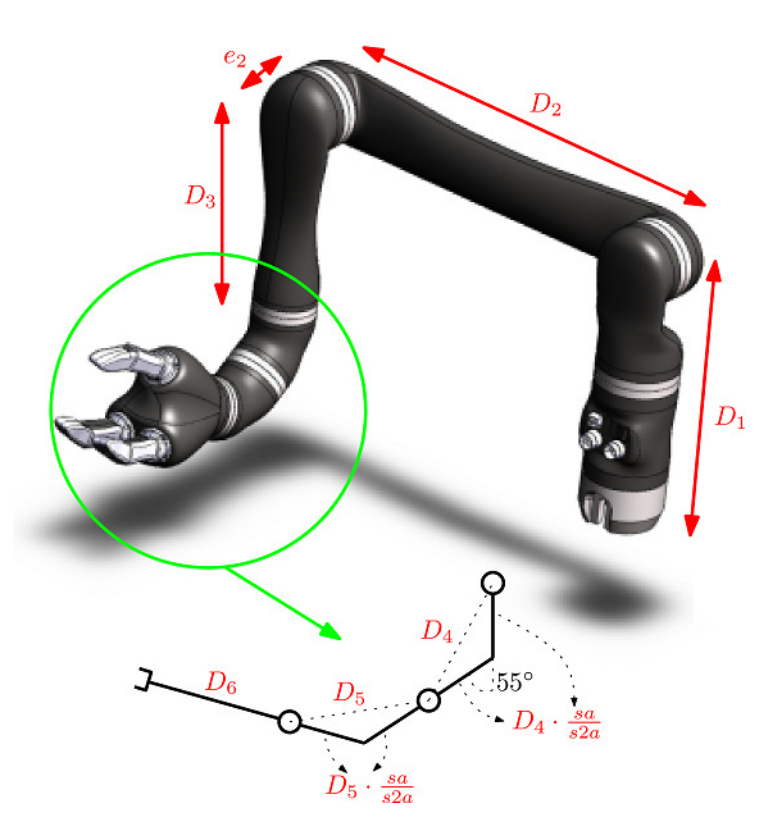
\includegraphics[scale=0.35]{jacoDH1}
\caption{Model Jaco robotske ruke sa označenim parametrima} \label{jacoparam}
\end{figure}

\begin{table}[h!]
    \centering
    \begin{tabular}{ | l | l | l |}
    \hline
    $D_{1}$ & $0.2755$ [m] \\ \hline
    $D_{2}$  & $0.4100$ [m] \\ \hline
    $D_{3}$  & $0.2073$ [m] \\ \hline
    $D_{4}$  & $0.0743$ [m] \\ \hline
    $D_{5}$  & $0.0743$ [m] \\ \hline
    $D_{6}$  & $0.1687$ [m] \\ \hline
    $e_{2}$  & $0.0098$ [m] \\ \hline
    $a$  & $\frac{11\cdot\pi}{72}$ [m] \\ \hline
    $d_{4b}$  & $D_{3}+D_{4}\frac{\sin(a)}{\sin(2a)}$ [m] \\ \hline
    $d_{5b}$  & $D_{4}+D_{5}\frac{\sin(a)}{\sin(2a)}$ [m] \\ \hline
    $d_{6b}$  & $D_{6}+D_{5}\frac{\sin(a)}{\sin(2a)}$ [m] \\ \hline
    \end{tabular}
    \caption{Konstrukcijski parametri Jaco robotske ruke}
\end{table}

\begin{equation}
d_{4b}=D_{3}+D_{4}\frac{1}{2\cdot\cos(a)}=D_{3}+D_{4}\frac{\sin(a)}{\sin(2a)}
\label{d4b}
\end{equation}
\begin{equation}
d_{5b}=D_{4}+D_{5}\frac{1}{2\cdot\cos(a)}=D_{4}+D_{5}\frac{\sin(a)}{\sin(2a)}
\label{d5b}
\end{equation}
\begin{equation}
d_{6b}=D_{6}+D_{5}\frac{1}{2\cdot\cos(a)}=D_{6}+D_{5}\frac{\sin(a)}{\sin(2a)}. 
\label{d6b}
\end{equation}

Ne ulazeći u pojedinosti DH metode, potrebno je napomenuti da $d$ i $a$ parametri predstavljaju međusobne odmake koordinatnih sustava zglobova, dok kut $\theta$ predstavlja rotaciju koordinatnih sustava oko vlastite osi rotacije. Navedenim parametrima dodajemo i razlike u orijentaciji rotacijskih osi zglobova $\alpha$:\\
 \begin{table}[h!]
\centering
\begin{tabular}{c c c c c}
\hline\hline
$ k $ & $ \alpha_{k} $ & $ a_{k} $ & $ d_{k} $ & $ \theta_{k} $ \\
%heading
\hline
1 & $ \pi/2 $ & $ 0 $ & $ D_{1} $ & $ \theta_{1} $\\
2 & $ \pi $ & $ D_{2} $ & 0 & $ \theta_{2} $\\
3 & $ \pi/2 $ & 0 & $ -e2 $ & $ \theta_{3} $\\
4 & $ \frac{11\pi}{36} $ & 0 & $ -d_{4b} $ & $ \theta_{4} $\\
5 & $ \frac{11\pi}{36}  $ & 0 & $ -d_{5b} $ & $ \theta_{5} $\\
6 & $ \pi $ & 0 & $ -d_{6b} $ & $ \theta_{6} $\\
\hline
\end{tabular}
\caption{DH parametri} \label{JacoDH}
\end{table}

Odnos kuteva u matematičkom modelu i stvarnih kuteva zglobova Jaco ruke dan je izrazima \ref{q1}, \ref{q2}, \ref{q3}, \ref{q4}, \ref{q5}, \ref{q6} :
 \begin{equation}
\theta_{1}=-q_{1_{Jaco}}
\label{q1}
\end{equation}
\begin{equation}
\theta_{2}=q_{2_{Jaco}}-\frac{\pi}{2}
\label{q2}
\end{equation}
\begin{equation}
\theta_{3}=q_{3_{Jaco}}+\frac{\pi}{2}
\label{q3}
\end{equation}
\begin{equation}
\theta_{4}=q_{4_{Jaco}}
\label{q4}
\end{equation}
\begin{equation}
\theta_{5}=q_{5_{Jaco}}-\pi
\label{q5}
\end{equation}
\begin{equation}
\theta_{6}=q_{6_{Jaco}}+\dfrac{5\cdot \pi}{9}
\label{q6}
\end{equation}\\

Varijabla $q_{i_{Jaco}}$ predstavlja trenutačnu rotaciju i-tog zgloba Jaco robotske ruke očitanu kroz API, dok $\theta_i$ predstavlja stvarni zakret i-tog zgloba.

\subsubsection{Matrice homogene transformacije}
Matrica homogene transformacije između dva koordinatna sustava postavljena prema D-H postupku određena je izrazom \ref{homogena}.
Vektor $\mathbf{p} = [x\ y\ z]^T$ sadrži poziciju ishodišta k-tog koordinatnog sustava u koordinatnom sustavu k-1.
Matrica $\mathbf{R}$ je matrica rotacije koja definira orijentaciju koordinatnog sustava k u koordinatnom sustavu k-1.
\begin{equation}
\mathbf{T_{k-1}^k} =
\begin{bmatrix} 
\mathbf{R} & \mathbf{p}\\ 
\mathbf{0} & 1\\
\end{bmatrix}
=
\begin{bmatrix} 
\cos\theta_{k}& -\cos\alpha_{k}\sin\theta_{k} & \sin\alpha_{k}\sin\theta_{k} & a_k\cos\theta_{k}\\ 
\sin\theta_{k}& \cos\alpha_{k}\cos\theta_{k} & -\sin\alpha_{k}\cos\theta_{k} & a_k\sin\theta_{k}\\
0 & \sin\alpha_{k} & \cos\alpha_{k} & d_{k}\\
0 & 0 & 0 & 1\\
\end{bmatrix}
\label{homogena}
\end{equation}

Uvrštavajući podatke iz tablice \ref{JacoDH} u izraz \ref{homogena} dobivamo matrice homogenih transformacija za koordinatne sustave Jaco robotske ruke.
\begin{equation}
\mathbf{T_0^1} =\begin{bmatrix} \cos\theta_{1}& 0 & \sin\theta_{1} & 0\\ 
\sin\theta_{1}& 0 & -\cos\theta_{1} & 0\\
0 & 1 & 0 & d_{1}\\
0 & 0 & 0 & 1\\
\end{bmatrix}
\end{equation}

\begin{equation}
\mathbf{T_1^2} =\begin{bmatrix} \cos\theta_{2}& \sin\theta_{2} & 0 & a_{2}\cos\theta_{2}\\ 
\sin\theta_{2}& -\cos\theta_{2} & 0 & a_{2}\sin\theta_{2}\\ 
0 & 0 & -1 & 0\\
0 & 0 & 0 & 1\\
\end{bmatrix}
\end{equation}

\begin{equation}
\mathbf{T_2^3} =\begin{bmatrix} \cos\theta_{3}& 0 & \sin\theta_{3} & 0\\ 
\sin\theta_{3}& 0 & -\cos\theta_{3} & 0\\
0 & 1 & 0 & d_{3}\\
0 & 0 & 0 & 1\\
\end{bmatrix}
\end{equation}

\begin{equation}
\mathbf{T_3^4} =\begin{bmatrix} \cos\theta_{4}& -\cos\alpha_{4}\sin\theta_{4} & \sin\alpha_{4}\sin\theta_{4} & 0\\ 
\sin\theta_{4}& \cos\alpha_{4}\cos\theta_{4} & -\sin\alpha_{4}\cos\theta_{4} & 0\\
0 & \sin\alpha_{4} & \cos\alpha_{4} & d_{4}\\
0 & 0 & 0 & 1\\
\end{bmatrix}
\end{equation}

\begin{equation}
\mathbf{T_4^5} =\begin{bmatrix} \cos\theta_{5}& -\cos\alpha_{5}\sin\theta_{5} & \sin\alpha_{5}\sin\theta_{5} & 0\\ 
\sin\theta_{5}& \cos\alpha_{5}\cos\theta_{5} & -\sin\alpha_{5}\cos\theta_{5} & 0\\
0 & \sin\alpha_{5} & \cos\alpha_{5} & d_{5}\\
0 & 0 & 0 & 1\\
\end{bmatrix}
\end{equation}

\begin{equation}
\mathbf{T_5^6} =\begin{bmatrix} \cos\theta_{6}& \sin\theta_{6} & 0 & 0\\ 
\sin\theta_{6}& -\cos\theta_{6} & 0 & 0\\ 
0 & 0 & -1 & d_{6}\\
0 & 0 & 0 & 1\\
\end{bmatrix}
\end{equation}

Množenjem ovih matrica dobivamo matricu homogene transformacije između baze robota i alata \ref{b-a}
\begin{equation}
\mathbf{T_{alat}^{baza}} = \mathbf{T_1^0}\ \mathbf{T_2^1}\ \mathbf{T_3^2}\ \mathbf{T_4^3}\ \mathbf{T_5^4}\ \mathbf{T_6^5}
\label{b-a}
\end{equation}

Članove ove matrice određujemo koristeći matlab skriptu, rezultat računa i skripta ispisani su u dodatku.
Iz matrice $\mathbf{T_{alat}^{baza}}$ dobivamo potpunu informaciju o položaju alata u baznom koordinatnom sustavu kao funkciju zakreta zglobova:
\begin{equation}
\mathbf{w}(\bm \theta) = 
\begin{bmatrix}
\mathbf{p}\\
\mathbf{r}(\mathbf{R})
\end{bmatrix}
\label{konfig_alat}
\end{equation}

Vektor \ref{konfig_alat} još nazivamo vektorom konfiguracije alata.

\subsection{Inverzna kinematika}
Ciljane konfiguracije izvršnog člana u $\mathbb{R}^{3}$ dane su vektorom $\vec{\mathbf{t}} = (\mathbf{t_1}, \ldots , \mathbf{t_k})^{T}$ , a trenutne konfiguracije vektorom
$\vec{\mathbf{w}} = (\mathbf{w_1}, \ldots , \mathbf{w_k})^{T}$. Kod mehaničkih manipulatora , $\vec{\mathbf{w}}$ je funkcija pozicija zglobova ${\bm{\theta}} = (\theta_{1}, \ldots , \theta_{n})^{T}$ , pa za ovaj slučaj zapisujemo $\vec{\mathbf{w}}=\vec{\mathbf{w}}\left({\vec{\bm{\theta}}}\right) $ . Problem inverzne kinematike definiramo kao pronalaženje vektora $\vec{\bm{\theta}} = (\bm{\theta_1} \ldots \bm{\theta_k})^T$ koji zadovoljava izraz:
\begin{equation}
\mathbf{t_i} = \mathbf{w_i}(\bm{\theta}_{\mathbf{i}})
\label{inverzna_def}
\end{equation}

Ono što čini problem inverzne kinematike problemom u užem smislu jest netrivijalnost rješavanja sustava jednadžbi \ref{inverzna_def} kako bi dobili $\bm{\theta}_{\mathbf{i}}(\mathbf{t_i})$. 
Razvijeni su različiti pristupi ovom problemu od kojih se mnogi oslanjaju na numeričke metode ili metode pronalaženja minimuma odgovarajuće funkcije.

Korištenjem analitičke metode rješavanja opisane u uvodu ovog poglavlja, vektor $\bm{\theta}_{\mathbf{i}}(\mathbf{t_i})$ dobiva se rješavanjem sustava jednadžbi dobivenog iz vektora konfiguracije alata \ref{konfig_alat}. 
Promatrajući puni izraz za vektor konfiguracije alata $\mathbf{w}$, primjećujemo da je analitičko rješavanje ovog problema vrlo složen zadatak čije poopćavanje zahtjeva iznimno složen algoritam.
Ovo nas dovodi do zaključka da univerzalni algoritam rješavanja inverzne kinematike zahtjeva drugačiji pristup.

\section{Iterativno rješavanje kinematičkog problema}
Kako bi izbjegli komplicirano analitičko rješavanje problema inverzne kinematike, razvili smo metodu koja zaobilazi rješavanje sustava jednadžbi \ref{inverzna_def}.
Prvi se korak sastoji od određivanja matrice Jakobijana manipulatora, koja povezuje brzine okretanja zglobova sa linearnim i rotacijskim brzinama alata.

Pronalaženjem inverza ove matrice, moguće je odrediti potrebne brzine rotacije zglobova kako bismo ostvarili željene brzine gibanja alata.
Sintezom upravljačke petlje moguće je ostvariti praćenje referentne veličine u obliku zadanog vektora konfiguraciije alata, čime ostvarujemo iterativni postupak rješavanja inverzne kinematike.

\subsection{Jakobijan manipulatora}

Definiramo Jacobijevu matricu manipulatora kao promjenu vektora konfiguracije $\mathbf{w_i}$ u ovisnosti o promjeni $\bm{\theta}_{\mathbf{i}}$.
Radi jednostavnosti zapisa, u nastavku teksta ispuštamo indekse ovih vektora. Sada je izraz za Jacobijevu matricu:
\begin{equation}
\mathbf{J} =\frac{d\mathbf{w}}{d\bm{\theta}} 
\end{equation}

Počinjemo pretpostavkom da za dovoljno malene vrijednosti $\Delta \mathbf{w}$ vrijedi \ref{jac_approx}:
\begin{equation}
\Delta \mathbf{w} \approx \mathbf{J}  \Delta \bm{\theta}
\label{jac_approx}
\end{equation}

Inverzom matrice $\mathbf{J}$ možemo dobiti sljedeći vrlo koristan identitet:
\begin{equation}
\Delta \bm{\theta} \approx \mathbf{J}^{-1} \Delta \textbf{w}
\label{jac_approx2}
\end{equation}

Identitet \ref{jac_approx2} važan je jer zahvaljujući njemu ostvarujemo regulator brzine definiran u [poglavlje].

U generalnom slučaju Jacobijeva matrica predstavlja matricu dimenzija $n \times k$ gdje je $\mathbf{w_i} = (w_1, \ldots , w_k)^T$:
\begin{equation}
\mathbf{J} =
\begin{bmatrix}
    \dfrac{\partial {w_1}}{\partial \theta_{1}}      & \dfrac{\partial {w}_{1}}{\partial \theta_{2}}  & \dots & \dfrac{\partial {w}_{1}}{\partial \theta_{n}}  \\
    \dfrac{\partial{w}_{2}}{\partial \theta_{1}}      & \dfrac{\partial {w}_{2}}{\partial \theta_{2}}  & \dots & \dfrac{\partial {w}_{2}}{\partial \theta_{n}} \\
    \vdots \\
    \dfrac{\partial {w}_{k}}{\partial \theta_{1}}      & \dfrac{\partial {w}_{k}}{\partial \theta_{2}}  & \dots & \dfrac{\partial {w}_{k}}{\partial \theta_{n}}
\end{bmatrix}
\end{equation}

U slučaju kada ova matrica predstavlja manipulator, vrijedi $k=6$.
Ove parametre ponekad nije jednostavno analitički odrediti, stoga je korištena geometrijska metoda kojom zaobilazimo deriviranje. 
Neka je $\mathbf{p}_{j}$ pozicija j-tog zgloba u baznom koordinatnom sustavu i neka je $\mathbf{z}_{j}$ jedinični vektor osi rotacije j-tog zgloba. 
Komponente rotacijskog dijela Jakobijana $J_{\bm{\omega}_j}$ jednake su jediničnim vektorima osi rotacije zgloba: 
\begin{equation}
J_{\bm{\omega}_j} = \dfrac{\partial \textbf{w}}{ \partial \theta_{j}} = \textbf{z}_{j}
\end{equation}


Uz pretpostavku da je rotacija mjerena u radijanima i da je smjer rotacije određen pravilom desne ruke , za translacijski dio Jakobijana $J_{\bm{v}_j}$ članovi iznose:
\begin{equation}
J_{\bm{v}_j} = \dfrac{\partial \mathbf{w}}{ \partial \theta_{j}} = \mathbf{z}_{j} \times (\mathbf{w} - \mathbf{p}_{j})
\end{equation}

U slučaju translacijskog zgloba, računanje člana još je jednostavnije jer je promjena pozicije jednaka jediničnom vektoru "osi rotacije" zgloba:
\begin{equation}
J_{\bm{v}_j} = \dfrac{\partial \mathbf{w}}{ \partial \theta_{j}} = \mathbf{z}_{j}
\end{equation}

Dobivena Jacobijeva matrica ima strukturu:
\begin{equation}
\mathbf{J} =
\begin{bmatrix}
J_{\bm{v}}\\
J_{\bm{\omega}}
\end{bmatrix}
\end{equation}

\begin{equation}
\mathbf{J} =
\begin{bmatrix}
\mathbf{z}_{0} \times (\mathbf{w} - \mathbf{p}_{0}) &\mathbf{z}_{1} \times (\mathbf{w} - \mathbf{p}_{1}) &\ldots &\mathbf{z}_{n-1} \times (\mathbf{w} - \mathbf{p}_{n-1})\\
\textbf{z}_{0} &\textbf{z}_{1} &\ldots &\textbf{z}_{n-1}\\
\end{bmatrix}
\end{equation}

Izrazom \ref{jac_approx2} lineariziramo model gibanja robota oko točke $\bm{\theta}$. 
Uz odgovarajuću frekvenciju osvježavanja matrice $\mathbf{J}$, moguće je dobiti kvalitetnu aproksimaciju $\Delta \bm{\theta}$ za željeni $\Delta \mathbf{w}$.
\newpage
\subsection{Upravljačka petlja}
%Pomoću izvedene Jakobijeve matrice manipulatora konstruiramo upravljačku petlju više razine koja regulira vektor konfiguracije alata $\mathbf{w}$.
Razmatranjem izraza \ref{jac_approx2} možemo zaključiti da smo posredno došli do alata za aproksimaciju inverzne kinematike. 
Iterativnom metodom moguće je ostvariti kretanje ruke prema željenoj točki dokle god poznajemo $\mathbf{e}$ . 
Ovom metodom pomoću već postojećih podataka možemo jednostavno dobiti rješenje za linearno kretanje bilo koje točke manipulatora.
\begin{figure}[!h]
\centering
\begin{tikzpicture}[auto, node distance=2cm,>=latex']
    % We start by placing the blocks
    \node [input, name=input] {};
    \node [sum, right of=input] (sum) {};
    \node [block, right of=sum] (Regulator) {{$\mathbf{J^{-1}}$}};
    \node [block, right of=Regulator, node distance=3cm] (system) {{manipulator}};
    % We draw an edge between the controller and system block to 
    % calculate the coordinate u. We need it to place the measurement block. 
    \draw [->] (Regulator) -- node[name=u] {$\bm{\omega}$} (system);
    \node [output, right of=system, node distance=2cm] (output) {};
    \node [block, below of=u] (measurements1) {$\mathbf{f}$};
    \node [block, below of=measurements1] (measurements) {$\mathbf{DK}$};

    % Once the nodes are placed, connecting them is easy. 
    \draw [draw ,->] (input) -- node {$\mathbf t$} (sum);
    \draw [->] (sum) -- node {$\mathbf{e}$} (Regulator);
    \draw [->] (system) -- node [name=y] {$\bm{\theta_r}$}(output);
    \draw [->] (y) |- (measurements);
    \draw [->] (y) |- (measurements1);
    \draw [->] (measurements) -| node[pos=0.99] {$-$} 
        node [near end] {$\mathbf w$} (sum);
    \draw [->] (measurements1) -| node[pos=0.99] {} 
        node [near end] {$\bm{\theta}$} (Regulator);    
\end{tikzpicture}
\caption{Blok dijagram izvedbe upravljače petlje manipulatora} \label{petlja}
\end{figure}

Definiramo vektor razlike konfiguracija kao: 
\begin{equation}
{\mathbf{e_i}} = {\mathbf{t_i}} -{\mathbf{w_i}}
\label{e}
\end{equation}

U daljnjem razmatranju iz izraza \ref{e} ispuštamo indekse radi kompaktnosti.
Razliku referentnog i stvarnog vektora konfiguracije alata sustav prema izrazu \ref{jac_approx2} množimo inverzom matrice $\mathbf{J}$.
Kao rezultat množenja dobivamo potrebne zakrete zglobova $\Delta \mathbf{q}$.
Pošto su rezultirajući referentni zakreti zglobova znatno manji od njihove nominalne kutne brzine, možemo ih tretirati i kao referentne brzine:
\begin{equation}
\Delta \mathbf{q} \approx \bm{\omega}
\end{equation}

Vektor funkcija $\mathbf{f}$ u ovom slučaju označava preračunavanje kuteva očitanih sa manipulatora ruke $\bm{\theta_r}$ u kuteve koji odgovaraju postavljenom matematičkom modelu $\bm{\theta}$. 
Dobivene kuteve koristimo kako bi osvježili matricu $\mathbf{J}$ i kako bi dobili trenutni vektor konfiguracije alata $\mathbf{w}$. 
Iz \ref{petlja} primjećujemo kako se radi o strukturi sa P (proporcionalnim) regulatorom jediničnog pojačanja, no sustav je moguće proširiti složenijim oblicima regulatora. 

\newpage

\subsubsection{Provjera sustava}
Shemu sustava predloženu shemom \ref{petlja} provjeravamo u programskom paketu Matlab.
Prvi korak je rješavanje direktne kinematike te generiranje funkcije \verb|jacoFK| koja kao argumente prima zakrete zglobova $\mathbf{q}$,
a kao rezultat vraća vektor konfiguracija alata.
%\begin{equation}
%\alpha = atan2\left(\frac{r_{21}}{r_{11}}\right)
%\end{equation}
%\begin{equation}
%\beta = atan2\left(\frac{-r_{31}}{\sqrt{r_{32}^2 + r_{33}^2}}\right)
%\end{equation}
%\begin{equation}
%\gamma = atan2\left(\frac{r_{32}}{r_{33}}\right)
%\end{equation}
\begin{figure}[h!]
\centering
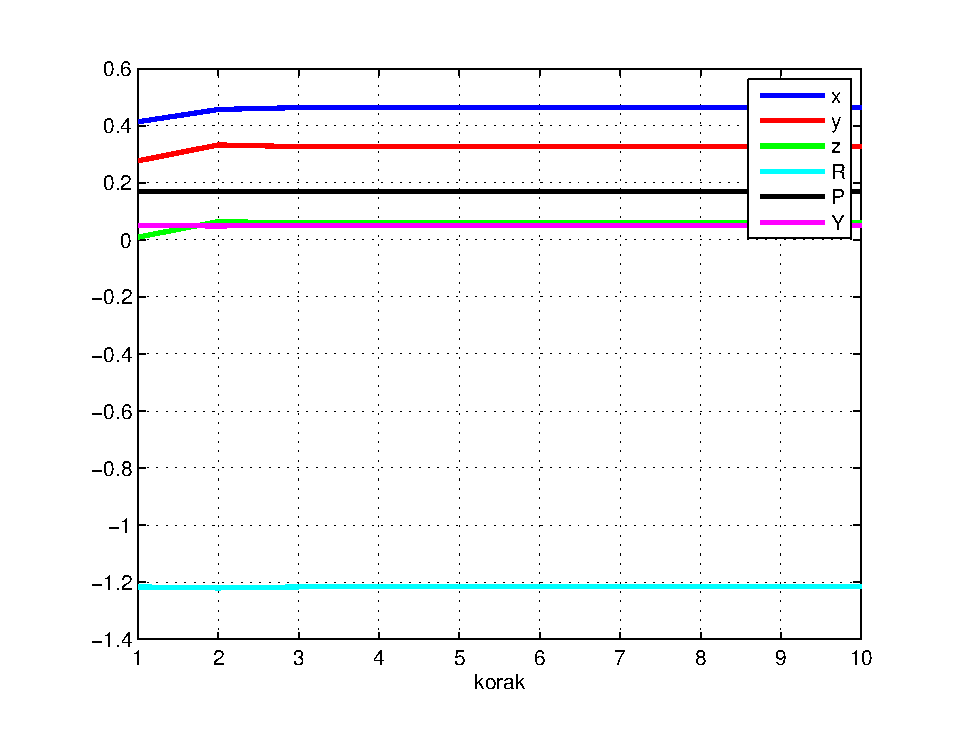
\includegraphics[scale=0.7]{P1}
\caption{Kretanje matematičkog modela Jaco robotske ruke za 5cm u smjeru x,y i z osi. Orijentacija alata je konstantna.} \label{P1}
\end{figure}

Iz grafa \ref{P1} vidljivo je kako pri čistom translacijskom kretanju upravljačka petlja sa P regulatorom ostvaruje željenu konfiguraciju unutar 3 koraka.
%ubaci vremena
Graf \ref{PPI} a) prikazuje ponašanje P upravljačke petlje pri složenijem gibanju koje obuhvaća i promjenu orijentacije.
Visoka razina oscilatornosti navodi nas na zaključak kako je za složenija gibanja potreban složeniji oblik regulatora.
\begin{figure}[h!]
\centering
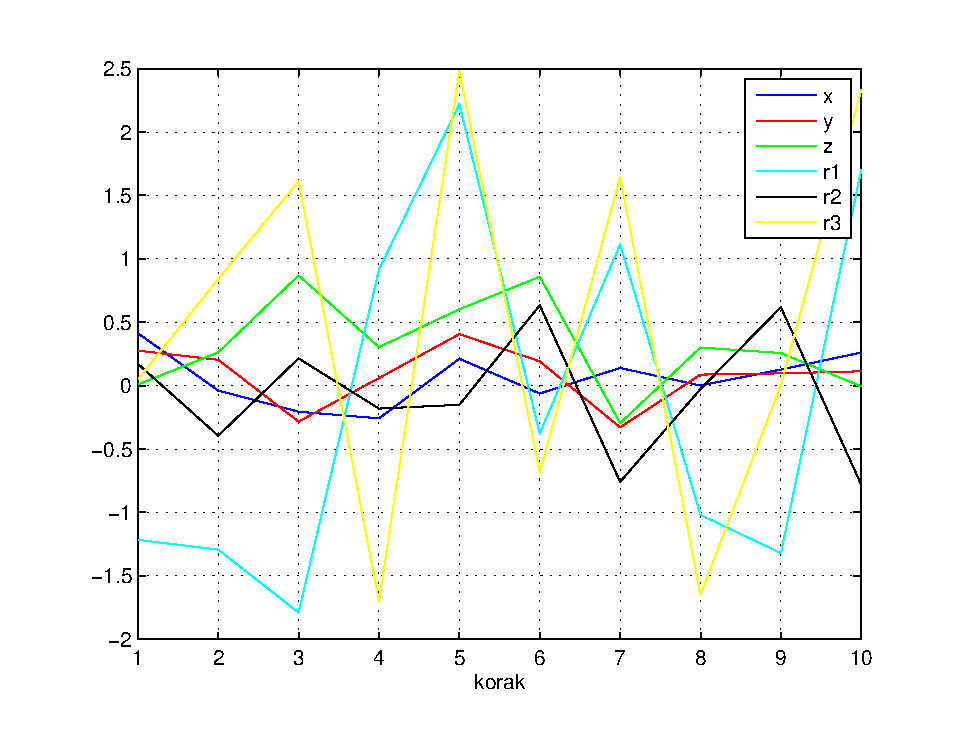
\includegraphics[width = 0.49\textwidth]{Preg}
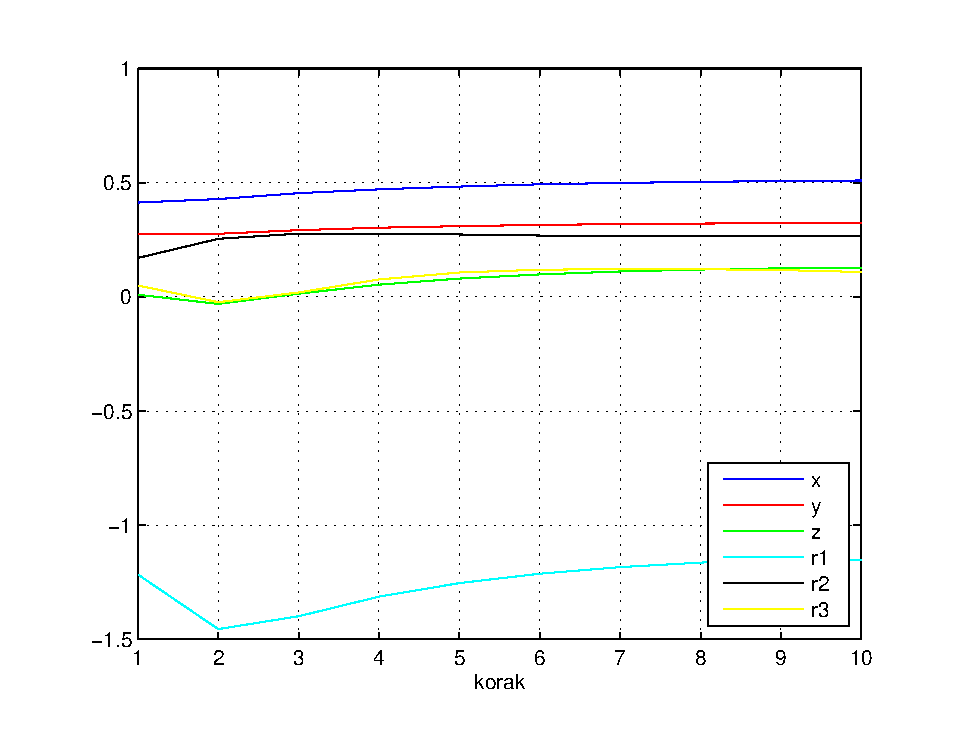
\includegraphics[width = 0.49\textwidth]{PIreg}
\caption{Odzivi upravljanja pri referentnoj konfiguraciji koja iziskuje regulaciju svih stupnjeva slobode.
Slika a) (lijevo) sadrži odziv sustava sa P regulatorom, b) (desno) sadrži odziv sustava sa PI regulatorom.} \label{PPI}
\end{figure}

Proporcionalno-integralnim (PI) regulatorom možemo značajno smanjiti oscilatornost sustava.
Pošto se regulator izvodi u kodu, potrebno ga je ostvariti rekurzivno:
\begin{equation}
\mathbf{u}(i)  = K_I\mathbf{u}(i-1) + K_I[\mathbf{e}(i) - \mathbf{e}(i-1)] + K_P\mathbf{e}(i)
\end{equation}

Parametriranje regulatora ostvarujemo pomoću optimizacije kriterijske funkcije \ref{krit} koja kažnjava oscilatornost i vrijeme potrebno za postizanje stacionarnog stanja.
\begin{equation}
crit(k) = crit(k-1) + 100 k (\mathbf{t} - \mathbf{w}(k)) (\mathbf{t} - \mathbf{w}(k))^T
\label{krit}
\end{equation}

Kako bi pronašli parametre $K_I$ i $K_P$ kojima ostvarujemo minimum ove funkcije koristimo Matlab funkciju \verb|fminsearch|.
Rezultirajući odziv matematičkog modela na grafu \ref{PPI} b) znatno je stabilniji korištenjem PI regulatora sa parametrima $[K_I \ K_P] = [ -0.2154  \  0.3197]$.
Potrebno je uzeti u obzir činjenicu da u ovom procesu nismo modelirali ponašanje samih elektromotora u zglobovima jer pretpostavljamo da su kvalitetno regulirani od strane FPGA pločice na samom manipulatoru. 
Ovi parametri također ovise o Jakobijanu korištenog manipulatora, ali u ovom potpoglavlju dovoljno nam je bilo dokazati da predložena struktura radi.

\chapter{Detekcijski algoritam}\label{Detekcijski algoritam}
Upravljanje pokretima ruke može se izvesti na više načina. U ovom radu odlučeno je koristiti dubinsku kameru kojom se snimaju čovjekovi pokreti ruke te se svaka snimljlena slika prevodi u informaciju o trenutnoj lokaciji i orijentaciji ruke u trodimenzionalnom prostoru kojeg dubinska kamera promatra.\\\\
Problem detekcije poze u kojoj se nalazi ruka s nekom dozom uspješnosti riješen
je i kod klasičnih slika (npr. //todo 3 citata), ali taj pristup većinom obilježava prevelika
ovisnost o svjetlosnim parametrima slike te potreba za većim računalnim resursima. Takvi zahtjevi otežavaju detekciju u stvarnom vremenu na osobnom računalu.\\\\
Većina pristupa detekciji objekata kod klasične slike s intenzitetom svjetlosti u pojedinim točkama može se primijeniti i kod dubinske slike. Pri tome dubinsku sliku možemo promatrati kao klasičnu sivu sliku te raditi detekcije nad istom samo moramo imati na umu kako informacija koju sadrži pojedini slikovni element ne odgovara intenzitetu, već je mjera udaljenosti. Također uobičajena crno-bijela slika se sastoji od 8-bitnih vrijednosti što polučuje 256 različitih slikovnih elemenata te u većini slučaja možemo biti zadovoljni s tim. Kod dubinske slike to nije slučaj. Ako imamo 256 različitih slikovnih elemenata sposobni smo detektirati 256 različitih dubina, s čime ne možemo biti zadovoljni ako želimo detekciju na većem rasponu (1m) uz veliku preciznost (1mm). Zato je uobičajen zapis dubinske slike
pomoću 2 okteta ili broja s jednostrukom preciznosti po IEEE 754 standardu. Ovaj
potonji zapis kompatibilan je s korištenom OpenCV bibliotekom.\\\\
Razvijeni detekcijski algoritam podijeljen je u dvije slijedne komponente. Lokalizacija dlana  u slici te određivanje parametara poze u kojoj se dlan nalazi.\\\\
\section{Lokalizacija dlana u slici}
Jednako kao i kod klasičnih slika prvi korak u preciznom detektiranju poze u kojoj se nalazi ruka jest određivanje njene lokacije na dubinskoj slici. Različite metode su predložene za rješavanje takvog problema. Pri tome rijetko koja metoda ne koristi neki oblik pomagala kako bi što lakše i brže odredila lokaciju u dubinskoj slici te više vremena mogla posvetiti samom određivanju poze u kojoj se ruka nalazi.\\\\
Kako se ovaj rad orijentira na dubinske slike, a ne klasične slike s dodanim dubinskim kanalom, takvi pokušaji su zanemareni, ali valja spomenuti kako se filtriranjem isključivo boje kože može olakšati pretraga ruke. Neki od takvih pristupa koriste brzu detekciju lica i uzorkovanje parametara boje kože detektirane osobe radi poboljšavanja filtera boje pomoću dobivenih parametara.\\\\
\subsection{Slične metode}
Qian i suradnici razvili su jednu od najkvalitetnijih metoda danas \cite{qian2014realtime}. Metoda inicijalno pretpostavlja kako se ruka nalazi najbliže kameri u odnosu na ostale objekte u dubinskoj slici. Također, pretpostavlja korištenje nereflektirajuće narukvice na zapešću kojom se lako može izolirati ruka od okoline algoritmom poplavljivanja interesnog područja (eng. \textit{flood fill}).\\\\
Bolja inicijalna metoda preuzeta je iz rada Shottona i suradnika \cite{shotton2013real} u kojem detektiraju položaj čovjeka na dubinskoj slici. Implementirano prepoznavanje ljudskog kostura pomoću Kinect uređaja temelji se na njihovoj metodi. Tu inicijalnu metodu koriste Thompson i suradnici \cite{tompson2014real}. Metoda koristi jednostavne značajke $f_{\theta}(I,\mathbf{x})$ za svaki slikovni element $\mathbf{x}$ koje su invarijantne na dubinu $d_{I}(\mathbf{x}) $ (Izraz \ref{eq:depth_invariant_feature}).
\begin{equation}\label{eq:depth_invariant_feature}
f_{\theta}(I,\mathbf{x})=d_{I}(\mathbf{x}+ \frac{\mathbf{u}}{d_{I}(\mathbf{x})})-d_{I}(\mathbf{x}+ \frac{\mathbf{v}}{d_{I}(\mathbf{x})})\end{equation}
Dalje za svaki slikovni element $\mathbf{x}$ učenjem šume nasumičnih stabala odluke (eng. \textit{random decision forrest}) odredi se svega nekoliko parova odmaka $(\mathbf{u},\mathbf{v})$ koji dobro binarno klasificiraju svaki slikovni element pripada li on naučenom skupu objekata ili ne.\\\\
Grupiranjem slikovnih elemenata koji su imali pozitivan odziv klasifikatora možemo izolirati ruku ili više njih na dubinskoj slici.\\\\
Iako je metoda uspješna i relativno brza, pogotovo na grafičkoj kartici za koju je primarno namijenjena, u slučaju ovog završnog rada nedostatak takve metode bilo bi trajanje njenog učenja. Naime, autori navode kako na klasteru od 1000 jezgara učenje šume od 3 stabla do dubine 20 traje 1 dan, a uzevši u obzir nedostatak navedenih resursa, takav pristup u ovom radu nije moguć.\\\\
\subsection{Razvijena metoda}

Dubinska slika kakvu stvara korištena dubinska kamera je veličine 640x480 slikovnih elemenata. Pri tome vrijednost svakog slikovnog elementa odgovara izračunatom disparitetu na toj poziciji. Pomoću \textit{freenect} biblioteke takav podatak se može pretvoriti u dubinu u milimetrima.\\\\
Definiran je koordinatni sustav sa središtem u očištu kamere i osima $x$ i $y$ s odgovarajućim indeksom $(u+320,v+240)$ slikovnog elementa (kako bi središte koordinatnog sustava pomakli u središte slike). Osi x i y su skalirane na odmak od središta u milimetrima. Os z odgovara dubini slike također u milimetrima. Prirodom perspektivne projekcije kakvu daje dubinska kamera udaljenost od kamere ne odgovara udaljenosti do projekcijske ravnine. Samim tim se ne može izravno preslikati u z-os koordinatnog sustava, ali kako dlan na radnim udaljenostima ne zauzima više od 15\% slike na tom području je aproksimacija prihvatljiva.\\\\
Jedna od mogućih aproksimativnih formula za preslikavanje dispariteta u udaljenost od kamere, kakvu koristi \textit{freenect} biblioteka \cite{openkinect} je sljedeća (Izraz \ref{eq:approx_raw_disparity_to_mm}):
\begin{equation}
	\label{eq:approx_raw_disparity_to_mm}
	z_{d}(\mathbf{x})=\frac{1000}{-0.00307*d(\mathbf{x})+3.33}
\end{equation}
Dobivenim vrijednostima dubine možemo izračunati $x$ i $y$ vrijednosti koordinantnog sustava na sljedeći način:
\begin{equation}
	\label{eq:raw_disparity_to_mm_x}
	    x(z,u)=0.0021(v - 320)(z-10) 
\end{equation}
\begin{equation}
	\label{eq:raw_disparity_to_mm_y}
	    y(z,v)=0.0021(v - 240)(z-10)
\end{equation}
Kao i kod metode Qiana i suradnika \cite{qian2014realtime}, ali i mnogih drugih, i u ovom radu se pretpostavlja kako se ruka nalazi na najmanjoj dubini (niti jedan predmet u vidnom polju kamere nije bliži od ruke).\\\\

Za razliku od spomenute metode, u ostvarenoj metodi nije potrebno koristiti pomagala kao što je nereflektirajuća crna narukvica na zapešću. Izolacija dlana od okoline vrši se jednostavnim dubinskim filterom na empirijski određenoj dubini od $110mm$ u odnosu na globalni minimum dubine slike, što je ujedno i globalni minimum dijela slike na kojem se nalazi ruka. Iako najveći raspon prosječne ruke premašuje $110mm$, to ne predstavlja prevelik problem.\\\\
Na slikama \ref{fig:successful_palm_isolation} vidimo primjere ispravne izolacije dlana na dubinskoj slici. Radilo se o uspravnom dlanu (a), dlanu s dorzalne strane (b), pa čak dlanu u vodoravnoj ravnini (c) ili zatvorenom dlanu (d), ovakav jednostavni detektor je sposoban razlučiti dlan kako bi što više procesnog vremena mogao prepustiti sljedećim fazama detekcije.\\\\

U nekim slučajevima detekcija nije ispravna, ali je u granicama otpornosti kasnijih faza detektora. Tako se pri većim kutovima dlana u odnosu na projekcijsku ravninu mogu desiti dva slučaja (Slika \ref{fig:satisfactorily_palm_isolation}). Ako je najbliža točka dlana na području zapešća, zahvaćen je i dio podlaktice, dok ako je najbliža točka na području prstiju, dlan djelomično izlazi iz granica dubinskog filtera.\\\\
Oba slučaja većinom ne predstavljaju prevelik problem, no postoje i neke iznimke. Naime, ako je podlaktica u razini dlana, detektor neće biti sposoban razlučiti dlan od podlaktice (Slika \ref{fig:poor_palm_isolation}). Takav slučaj predstavlja problem za detektor, ali takav slučaj ne predstavlja problem u korištenju detektora ako je osoba koja ga koristi svjesna takvog nedostatka.\\\\
Rezultat izolacije dlana uz sliku na kojoj se nalazi samo dlan je i $(x,y,z)$ koordinata središta dlana u prostoru. Središte je dobiveno pronalaskom konture dlana te izlučivanjem njenog središta. Prije pronalaska konture na binarnoj slici se izvodi morfološka operacija zatvaranja s jezgrom veličine u radijusu od 2 susjedna slikovna elementa (Manhattan udaljenost). U slučaju da je središte konture izvan konture pa samim time i dlana, takva detekcija biva odbačena. Iako postoje položaji ruke gdje je to slučaj, takve položaje u većini slučajeva Kinect nije sposoban registrirati (Poglavlje \ref{sec:kinect_depth}).\\\\
Jednom kada je dlan segmentiran od pozadine znatno se olakšavaju daljnje operacije. Za razliku od spomenutih naprednijih radova ovdje se neće razmatrati određivanje precizne lokacije ruke u vidu modela od više od 20 stupnjeva slobode. Naime, uzevši u obzir primjenu detektora za upravljanje robotskom rukom, prihvatljiva doza informacije sastoji se od binarne informacije o stupnju zatvorenosti dlana i radij vektora lokacije dlana te eventualno orijentacija dlana u smjeru x-osi definiranog koordinatnog sustava.\\\\

Neki od ključnih postupaka u detekciji izvedeni su pomoću biblioteke OpenCV:
\begin{enumerate}[label=$\bullet$]
	\item \textbf{Segmentacija slike na osnovu praga} je postupak prilikom kojeg se s obzirom na željenu vrijednost praga može konstruirati binarna slika (maska) gdje jedna vrijednost pokriva sve elemente čija je vrijednost ispod praga, a druga vrijednost sve elemente iznad praga. Na slici \ref{fig:image_segmentation} (b) vidimo binarnu sliku dobivenu segmentacijom po dubini slike (a) pri čemu je prag određen kao $110mm$ u dubinu od minimalne vrijednosti dubine na slici.
\item \textbf{Dilatacija i erozija binarne slike} su morfološke transformacije. Dilatacija je transformacija prilikom koje se generira nova slika iste veličine. Za svaki osvijetljeni slikovni element u početnoj slici se u ovoj slici osvjetljava element na toj lokaciji zajedno s $n$ slikovnih elemenata u njegovoj okolini. Takvim postupkom smo povećali osvijetljene površine na slici. Erozija je slična dilataciji s razlikom što se postupak temelji na neosvijetljenim slikovnim elementima.\\\\
Na slici \ref{fig:morph} (c) je prikazana morfološka transformacija izvorne slike (a) operacijom zatvaranja (dilatacija pa erozija) uz djelovanje na okolnih 8 slikovnih elemenata. Kao što vidimo ovakav slijed transformacija pokriva moguće šumove unutar osvijetljenog dijela slike te može spojiti bliske skupine osvijetljenih slikovnih elemenata što je korisno ako na primjer šum \textit{odsiječe} prst od ostatka ruke.\\\\
\item \textbf{Određivanje obujmica} skupina osvijetljenih slikovnih elemenata koristan je način za aproksimaciju oblika na slici. Prvi korak u određivanju obujmica (engl. \textit{convex hull}) je generiranje kontura oko skupina susjednih slikovnih elemenata. Jednom kada je kontura izgenerirana jednostavno se može naći obujmica kao minimalan konveksan poligon koji obuhvaća konturu.\\\\
Na slici \ref{fig:convex_hull} je običnoj binarnoj slici sivom bojom pridodana razlika u površini konture oblika i obujmice. Ta razlika se može iskoristiti kao dobar indikator zatvorenosti dlana.

\end{enumerate}
\section{Određivanje poze dlana}

\subsection{Slične metode}
Različiti radovi predlažu različite metode određivanja poze u kojoj se nalazi ruka, ali i u različitom opsegu preciznosti.\\\\
Qian i suradnici u svom radu \cite{qian2014realtime} su modelirali prosječnu ruku pomoću 48 sfera uz 26 stupnjeva slobode. Pretražuju ekstreme u području dlana te im oni služe kao kandidati za vrhove prstiju i zapešće. Pomoću inverzne kinematike nad modelom generiraju moguće položaje ruke te svaki od njih ocjenjuju s obzirom na sličnost s dubinskom slikom. Najbolji model je proglašen trenutnim položajem ruke.\\\\
Thompson i suradnici u svojem radu \cite{tompson2014real} koriste naučenu kaskadu konvolucijskih neuronskih mreža. Učenje je izvršeno na 70 000 označenih slika. Mreže na izlazu daju dvodimenzionalnu Gaussovu razdiobu vjerojatnosti da se na određenoj lokaciji nalazi jedna od 36 označenih lokacija na ruci (npr. vrh malog prsta). I u ovom radu inverznom kinematikom se traži model ruke koji najviše odgovara razdiobama. Pri tome je rabljen često korišten model ruke otvorenog koda \textit{libhand} \cite{libhand}.\\\\
Valja napomenuti kako su navedene metode sposobne prepoznati ruku u jednoj dubinskoj slici te im ne treba niz slika.

\subsection{Razvijena brza metoda određivanja zatvorenosti dlana}
Zatvorenost dlana je apstraktan pojam te ga treba pobliže definirati. Prilično je intuitivan pojam otvoreni dlan koji predstavlja dlan u planarnom položaju, pri čemu kutevi između članaka teže nuli (Slika \ref{fig:successful_palm_isolation} a). Isto tako je jasan je pojam zatvorenog dlana (Slika \ref{fig:successful_palm_isolation} d). Teško je pak definirati stupanj zatvorenosti prilikom neke geste, pri kojoj dlan nije ni potpuno otvoren ni zatvoren, pogotovo ako je svaki prst pod svojim kutom. Tako se u ovom radu stupanj zatvorenosti određuje binarno pri čemu \textit{0} predstavlja zatvoren dlan, a \textit{1} sve ostale položaje.\\\\
Navedeni pristup sasvim je dovoljan pri kontroli željenog robota jer takav klasifikator nam određuje hoće li se prsti robotske ruke skupiti ili ne. Naime, iako robot posjeduje prste, nezgrapno bi bilo odrediti parametar zatvorenosti za svaki prst kako broj robotskih prstiju (3) ne korespondira broju ljudskih.\\\\
Klasifikator je napravljen jednostavno i empirijski. Izračuna se površina binarne slike zahvaćena konturom dlana ($ P_{k}(\mathbf{s}) $) i površina obujmice iste konture ($ P_{o}(\mathbf{s}) $). Generira se značajka koja predstavlja omjer površine konture i obujmice (\ref{eq:closure_feature_1}).
\begin{equation}\label{eq:closure_feature_1}
f_{1}(\mathbf{s})=\frac{P_{k}(\mathbf{s})}{ P_{o}(\mathbf{s})} 
\end{equation}
Potom se normalizira površina konture kako bi bila invarijantna na dubinu te se ista tretira kao druga značajka (\ref{eq:closure_feature_2}).
\begin{equation}\label{eq:closure_feature_2}
f_{2}(\mathbf{s})={P_{k}}'(\mathbf{s}) 
\end{equation}
Određivanje zatvorenosti dlana vrši se određivanjem predznaka linearne kombinacije dvije navedene značajke te još ostaje samo odrediti parametre $k$ i $l$ (\ref{eq:closure_}).
\begin{equation}\label{eq:closure_}
Z(\mathbf{s})=\left\{\begin{matrix}
 1&  ako&kf_{1}(\mathbf{s})+lf_{2}(\mathbf{s})>0\\
 0& ako & kf_{1}(\mathbf{s})+lf_{2}(\mathbf{s})\leq 0
\end{matrix}\right.
\end{equation}
\subsubsection{Učenje klasifikatora}
Nakon što su definirane značajke, generirano je 2559 ispitnih primjera od kojih 1239 s otvorenim dlanom i 1320 sa zatvorenim dlanom. Grafikon 4.4 prikazuje točke koje predstavljaju slike u ravnini određenoj značajkama $f_{1}$ i $f_{2}$ s time da zatvoreni dlanovi su prikazani zelenom bojom, a otvoreni crvenom.\\\\
U ravnini značajki grafičkom metodom je aproksimiran pravac koji razdvaja dvije klase, zatvorene i otvorene dlanove s greškom od 3.4\%. Težilo se preciznijoj detekciji zatvorenog dlana, što je uzrokovalo gubitak u preciznosti detekcije otvorenog dlana. Takav pristup je vođen pretpostavkom da prilikom upravljanja robotskom rukom zatvoreni dlan podrazumijeva kako ruka drži neki objekt te želimo biti sigurni kako ga neće olako ispustiti bez naše volje. Iako za neki teži problem ovakav pristup detekciji otvorenosti dlana ne bi bio dobar te bismo se trebali okrenuti naprednijim metodama, u ovom slučaju rezultat je sasvim zadovoljavajuć s obzirom na poprilično jasnu distinkciju između dviju klasa.\\\\
Dobiveni pravac ima parametre $k = 0.67635$ i $l=0.035558$ koji se koriste u detektoru prilikom određivanja zatvorenosti dlana.


\chapter{Upravljački algoritam}\label{Upravljački algoritam}
Koristimo ranije objašnjene koncepte i metode kako bi detaljno objasnili arhitekturu i izvedbu upravljačke petlje.
U prvom potpoglavlju opisujemo sve uključene ROS čvorove, poruke i servise koji čine kostur upravljačkog algoritma.
Drugo potpoglavlje sadrži opis programskog rješenja kinematike izvedenog u KDL-u.

\begin{figure}[h!]
\centering
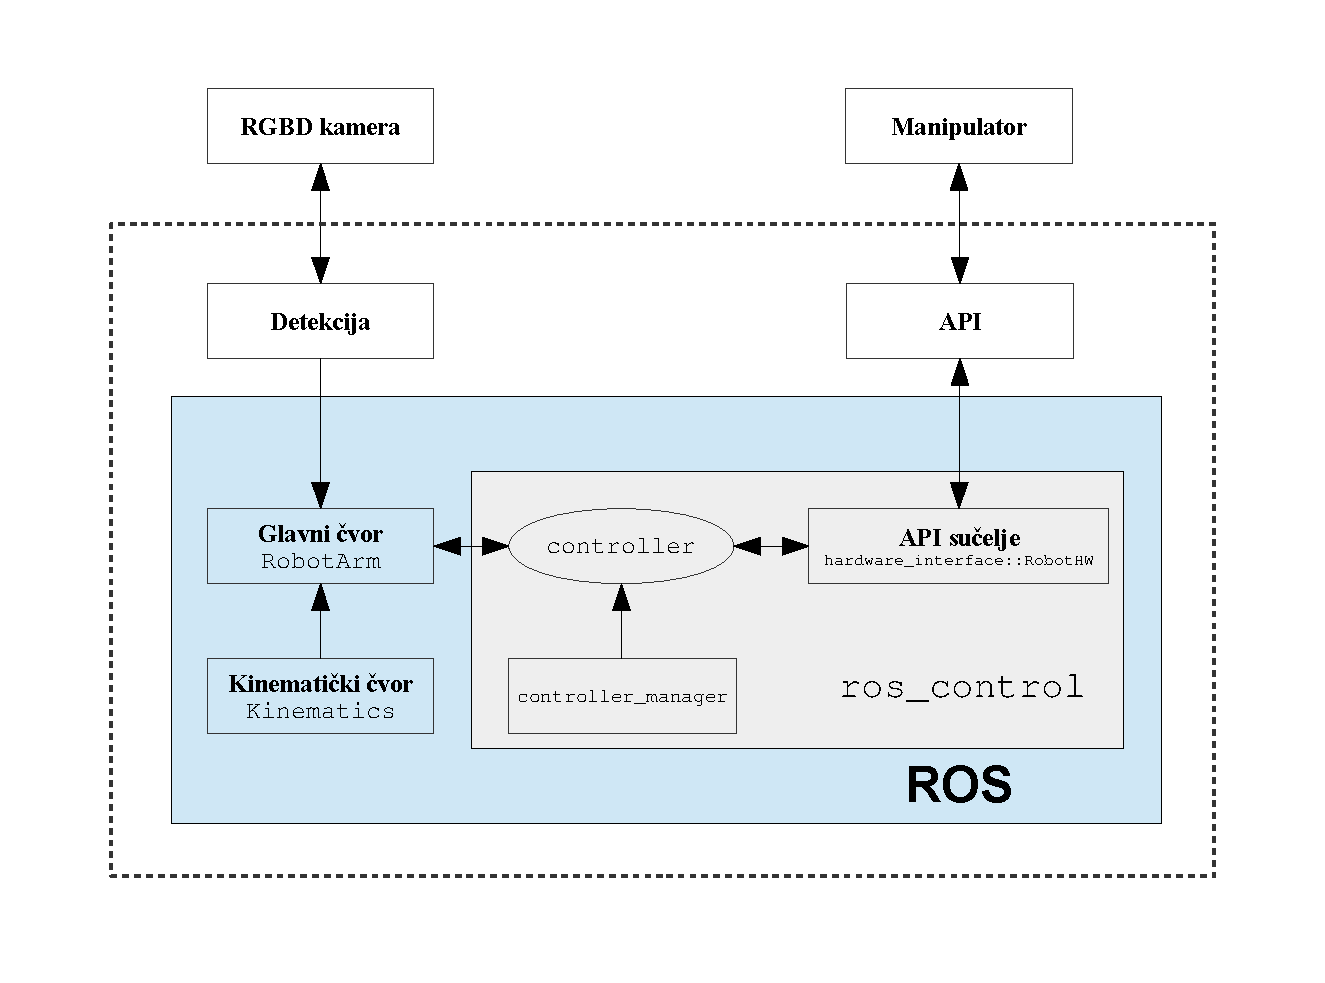
\includegraphics[width=\textwidth]{upr_shema}
\caption{Upravljačka shema}\label{upr_shm}
\end{figure}

Na slici \ref{upr_shm} prikazana je detaljna shema sustava u programskoj izvedbi.
Iscrtkani pravokutnik predstavlja granicu između uređaja i računala dok žuti i sivi predstavljaju područje sustava unutar ROS, odnosno \verb|ros_control| arhitekture, respektivno.


\section{Arhitektura upravljačke petlje}


\chapter{Rezultati}



\end{document}
